\chapter{Nominalflexion}

\label{sec:nominalflexion}
\index{Flexion}

Im Rahmen der Flexion -- also der Bildung der Wortformen von lexikalischen Wörtern (vgl.\ Kapitel~\ref{sec:morphologie}, Definition~\ref{def:flexion} auf S.~\pageref{def:flexion}) -- müssen für das Deutsche die \textit{Nomina} und die \textit{Verben} diskutiert werden.
Wortklassenfilter \ref{wfilt:flektierbare} (S.~\pageref{wfilt:flektierbare}) nahm schon (auf Umwegen) auf die Eigenschaft der Flektierbarkeit dieser beiden Klassen Bezug, ohne dass die genauen Einzelheiten besprochen wurden.
In diesem Kapitel geht es daher im Detail darum, wie die Wortformen der Nomina gebildet werden (\textit{Formseite}) und welche Markierungsfunktion diese Bildungen haben (\textit{Funktionsseite}).
Dies entspricht unserer Auffassung von Morphologie (Definition~\ref{def:morphologie}, S.~\pageref{def:morphologie}).%
\footnote{Die Nominalflexion wird auch mit dem Begriff der Lateingrammatik als \textit{Deklination} bezeichnet.}
Die Bedeutung soll so weit wie möglich nicht betrachtet werden (vgl.\ Abschnitt~\ref{sec:sprachealssymbolsystem}).
Dennoch wird bei der Beschreibung der Kategoriensysteme der Nomina (Abschnitt~\ref{sec:kategoriennomen}) relativ ausführlich auf die Motivation bestimmter Merkmale eingegangen, auch wenn diese Motivation teilweise semantisch ist.

Das Kapitel gliedert sich in die Beschreibung der nominalen Kategorien in Abschnitt~\ref{sec:kategoriennomen}, gefolgt von einer Diskussion der Substantive in Abschnitt~\ref{sec:subst}, der Artikel und Pronomina in Abschnitt~\ref{sec:artikelpronomen} und der Adjektive in Abschnitt~\ref{sec:adjektive}.
Der Begriff \textit{Nomen} ist gemäß Kapitel~\ref{sec:wortklassen} ein Oberbegriff für die Wörter, die zwar flektieren, aber nicht nach Tempus (und anderen typisch verbalen Kategorien).
Als Unterklassen werden gewöhnlich Substantive, Artikel, Pronomina und Adjektive definiert.
Einerseits müssen wir die Pronomina und die Artikel noch genau voneinander trennen (s.\ Abschnitt~\ref{sec:artikelpronomen}), andererseits soll hier zunächst überlegt werden, welche Merkmale die Nomina gemeinsam haben, und welchen funktionalen Kategorien oder Bedeutungskategorien diese Merkmale entsprechen.
Schon in Kapitel~\ref{sec:grundbegriffe} wurden Merkmale wie \textsc{Kasus} und \textsc{Numerus} ohne Definition oder argumentative Einführung benutzt.
In Abschnitt~\ref{sec:kategoriennomen} werden daher alle einschlägigen nominalen Merkmale systematisch angesprochen.
Zuvor muss allerdings mit Definition~\ref{def:vollstaendigesnominal} der Begriff der \textit{Nominalphrase} eingeführt werden, den wir im Rahmen der Flexion als Hilfsbegriff benötigen.
In Abschnitt~\ref{sec:ngr} wird dann eine allgemeinere Form der Nominalphrase eingeführt.


\index{Nominalphrase}

\Definition{Nominalphrase (vorläufig)}{\label{def:vollstaendigesnominal}%
Eine \textit{Nominalphrase} (NP) ist eine zusammenstehende Gruppe aus einem Substantiv, eventuell davor stehenden Adjektiven und einem eventuell davor stehenden Artikelwort.
Das Vorhandensein von Adjektiven und Artikelwort bedingt sich nicht gegenseitig.
Alle Nomina innerhalb der NP kongruieren in Genus, Kasus und Numerus.
}

Die in (\ref{ex:flex8882}) eingeklammerten Gruppen sind also NPs.

\begin{exe}
  \ex\label{ex:flex8882}
  \begin{xlist}
    \ex{\label{ex:flex8882a} [Gewichtheberinnen] haben [ein hartes Trainingsprogramm].}
    \ex{\label{ex:flex8882b} [Trainierte Gewichtheberinnen] haben [Chancen]\\auf [die Goldmedaille].}
    \ex{\label{ex:flex8882c} [Eine hervorragende Gewichtheberin] wurde [Olympiasiegerin].}
  \end{xlist}
\end{exe}


\section{Kategorien}

\label{sec:kategoriennomen}

\subsection{Numerus}

\label{sec:numerus}

\index{Numerus!Nomen}

Fast alle Nomina sind in irgendeiner Weise für \textsc{Numerus} spezifizierbar und weisen mehr oder weniger deutliche morphologische Numerusmarkierungen auf.
\textsc{Numerus} ist ein tendentiell semantisch motiviertes Merkmal mit im Deutschen zwei möglichen Werten, \textit{singular} (\textit{sg}) und \textit{plural} (\textit{pl}).
\textit{Semantische Motivation} bedeutet hier, dass es von den zu beschreibenden Sachverhalten in der Welt und nicht von grammatischen Bedingungen abhängt, ob eine Singular- oder eine Pluralform gewählt wird.
Die Sätze in (\ref{ex:flex3294}) sind lediglich durch den Numerus der jeweils zweiten NPs unterschieden, und sie beschreiben genau deswegen zwei verschiedene Sachverhalte.
Die Grammatik selbst liefert keine Kriterien zur Entscheidung, welcher der beiden Sätze in einer bestimmten Situation angemessen (oder wahr) ist, weshalb davon auszugehen ist, dass die Kategorie Numerus außerhalb der Grammatik semantisch motiviert ist.

\begin{exe}
  \ex \label{ex:flex3294}
  \begin{xlist}
    \ex{Die Trainerin beobachtet den Wettkampf.}
    \ex{Die Trainerin beobachtet die Wettkämpfe.}
  \end{xlist}
\end{exe}


Numerus ist bei den Nomina prinzipiell nicht statisch, und Nomina innerhalb von NPs kongruieren in ihren \textsc{Numerus}-Merkmalen, vgl.\ (\ref{ex:flex9111}) und (\ref{ex:flex9112}).

\begin{exe}
  \ex \label{ex:flex9111}
  \begin{xlist}
    \ex[]{Die Trainerin beobachtet [einen guten Wettkampf].}
    \ex[*]{Die Trainerin beobachtet [einen guten Wettkämpfe].}
  \end{xlist}
  \ex \label{ex:flex9112}
  \begin{xlist}
    \ex[]{Die Trainerin beobachtet [einige gute Wettkämpfe].}
    \ex[*]{Die Trainerin beobachtet [einige gute Wettkampf].}
  \end{xlist}
\end{exe}

Es gibt aber bestimmte Artikel und Pronomina, die statische Singulare oder Plurale sind.
Einige Beispiele finden sich in (\ref{ex:flex7298})--(\ref{ex:flex7301}).

\begin{exe}
  \ex \label{ex:flex7298}
  \begin{xlist}
    \ex{ein = [\textsc{Numerus}: \textbf{\textit{sg}}]}
    \ex{Die Trainerin beobachtet eine Spielerin.}
  \end{xlist}
  \ex \label{ex:flex7299}
  \begin{xlist}
    \ex{einige = [\textsc{Numerus}: \textbf{\textit{pl}}]}
    \ex{Die Trainerin beobachtet einige Spielerinnen.}
  \end{xlist}
  \ex \label{ex:flex7300}
  \begin{xlist}
    \ex{zwei = [\textsc{Numerus}: \textbf{\textit{pl}}]}
    \ex{Die Trainerin beobachtet zwei Spielerinnen.}
  \end{xlist}
  \ex \label{ex:flex7301}
  \begin{xlist}
    \ex{viele = [\textsc{Numerus}: \textbf{\textit{pl}}] }
    \ex{Die Trainerin beobachtet viele Spielerinnen.}
  \end{xlist}
\end{exe}

\index{Singularetantum}
\index{Pluraletantum}

Bestimmte Substantive treten aus semantischen Gründen oder aus \textit{Idiosynkrasie} (wortspezifische Eigenheit) nur im Singular oder im Plural auf.\index{Idiosynkrasie}
Man spricht von sogenannten \textit{Singulariatantum} oder \textit{Pluraliatantum}, vgl.\ (\ref{ex:flex6662}) und (\ref{ex:flex6663}).%
\footnote{Im Singular lauten diese Wörter \textit{Singularetantum} bzw.\ \textit{Pluraletantum}.}

\begin{exe}
  \ex\label{ex:flex6662}
  \begin{xlist}
    \ex[]{Die Spielerinnen genießen die Ferien.}
    \ex[*]{Die Spielerinnen genießen die Ferie.}
  \end{xlist}
  \ex\label{ex:flex6663}
  \begin{xlist}
    \ex[]{Die Spielerinnen erfreuen sich bester Gesundheit.}
    \ex[*]{Die Spielerinnen erfreuen sich bester Gesundheiten.}
  \end{xlist}
\end{exe}

\index{Kongruenz!Numerus--}

Auch wenn \textsc{Numerus} ein semantisch motiviertes Merkmal ist, so zeigt sich doch an den in diesem Abschnitt zitierten Beispielen, dass er in diverse grammatische Regularitäten (\zB Kongruenz) verwickelt ist.
Das Merkmal \textsc{Kasus}, um das es im nächsten Abschnitt geht, ist insofern grundlegend anders, als es überwiegend strukturell und in einer geringeren Menge von Fällen semantisch motiviert ist.


\begin{Vertiefung}{Numeruskongruenz und Koordination}

\index{Koordination}

\noindent Im Fall einer sog.\ \textit{Koordinationsstruktur} mit Konjunktionen wie \textit{und} oder \textit{oder} (vgl.\ Abschnitt~\ref{sec:koor}) kongruieren die mit der Konjunktion verbundenen NPs in ihrem Numerus nicht miteinander.
In (\ref{ex:flex1414}) ist \textit{eine Trainerin} eine NP im Singular, \textit{viele Spielerinnen} allerdings eine im Plural.

\begin{exe}
  \ex{\label{ex:flex1414} [Eine Trainerin] und [viele Spielerinnen] kamen auf den Platz.}
\end{exe}

Bezüglich Kasus herrscht dennoch Übereinstimmung.
Beide mit \textit{und} verbundenen NPs stehen im Nominativ, da sie zusammen auf dieselbe syntaktische Weise auf das Verb \textit{kamen} bezogen sind.
Traditionell würde man sagen, dass sie zusammen das Subjekt des Satzes bilden, vgl.\ Abschnitt~\ref{sec:subjekt}.

\end{Vertiefung}

\subsection{Kasus}

\label{sec:kasus}

\index{Kasus}
\index{Kasus!Hierarchie}
\index{Grammatikerfrage}

Die sogenannten \textit{Grammatikerfragen} sind genau wie die Klatschmethode im Bereich der Silbenphonologie (Abschnitt~\ref{sec:silben}) oder die semantische Wortklassifikation (Abschnitt~\ref{sec:semantischeklassifikation}) eine vergleichsweise unzureichende Antwort auf eine grammatische Fragestellung.
Hier ist es die Frage nach der Bestimmung der Kasus.
Die Grammatikerfragen ermitteln den \textit{Wer-Fall} (Nominativ), \textit{Wen-Fall} (Akkusativ), \textit{Wem-Fall} (Dativ) und den \textit{Wes-Fall} (Genitiv) anhand einer Fragediagnostik wie in (\ref{ex:flex2772}) und (\ref{ex:flex2773}).

\begin{exe}
  \ex \label{ex:flex2772}
  \begin{xlist}
    \ex{Der Ball ging ins Aus.}
    \ex{Frage: Wer oder was ging ins Aus?\\
    Antwort: Der Ball.\\
    Schlussfolgerung: \textit{Der Ball} steht im Wer-Fall (Nominativ)}
  \end{xlist}
  \ex \label{ex:flex2773}
  \begin{xlist}
    \ex{Der Ball kollidierte mit dem Pfosten.}
    \ex{Frage: Der Ball kollidierte mit wem oder was?\\
    Antwort: Dem Pfosten.\\
    Schlussfolgerung: \textit{dem Pfosten} steht im Wem-Fall (Dativ)}
  \end{xlist}
\end{exe}

Das Hauptproblem der Grammatikerfragen ist, dass sie eine vollständige Beherrschung der Kasus-Flexion und der Kasusrektion\slash Valenz der Verben und Präpositionen voraussetzen.
Es ist offensichtlich, dass \zB Deutschlerner mit den Grammatikerfragen deshalb nichts anfangen können, weil die Beantwortung der Frage voraussetzt, dass der im entsprechenden syntaktischen Kontext geforderte Kasus und die mit diesem Kasus einhergehende Flexion bekannt sind, wenn der Kasus nicht sowieso direkt an der Form der Nomina ablesbar ist.
Am Beispiel von (\ref{ex:flex2773}) könnte man also genausogut an der Form des Artikels \textit{dem} ablesen, dass es sich um einen Dativ handelt.
In dem Moment, wo Informationen wie diese fehlen, kann weder die Grammatikerfrage beantwortet werden, noch die Form \textit{dem Pfosten} gebildet werden.


\begin{Vertiefung}{Satzglieder und Grammatikerfragen}

\noindent Die Grammatikerfragen setzen zusätzlich eine vollständige syntaktische Analyse voraus, die zumindest an Schulen im erstsprachlichen Grammatikunterricht nicht erfolgt.
Die Katastrophe in (\ref{ex:flex4444}) wurde von einem niedersächsischen Lehrer im Fach Deutsch in der Sekundarstufe I (im Jahr 2005) zur Frage, was der Kasus von \textit{Hut} sei, vertreten.
Der in der Akkusativ-NP enthaltene Genitiv wird nicht korrekt zugeordnet, weil irgendwie diffus über Bedeutung nachgedacht wird, und weil keine angemessene Konstituentenanalyse vor der Kasusbestimmung durchgeführt wird.

\index{Satzglied}

\begin{exe}
  \ex \label{ex:flex4444}
  \begin{xlist}
    \ex{\label{ex:flex4444a} Wir sehen den Hut des Mannes.}
    \ex{\label{ex:flex4444b} Wessen Hut sehen wir? -- Den Hut des Mannes. $\rightarrow$ \Ast Wes-Fall\slash Genitiv}
  \end{xlist}
\end{exe}

Wird der Genitiv in einem pränominalen Relativpronomen versteckt (vgl.\ Abschnitte~\ref{sec:prondefart} und~\ref{sec:relativsaetze}), ist mit den Grammatikerfragen endgültig nichts mehr anzufangen, die Form \textit{dess-en} ist hingegen für sich genommen eindeutig ein Genitiv, s. (\ref{ex:flex41034}).

\begin{exe}
  \ex{\label{ex:flex41034} Ich sehe den Mann, dessen Hut ich geklaut habe. }
\end{exe}

Die einzig zielführende Variante der Grammatikerfragen ist der Verzicht auf die Fragen an sich.
Im besten Fall ist an der Form der Nomina bereits der Kasus eindeutig erkennbar.
Dies ist nur bei voll flektierten Pronomina (oder entsprechenden Artikeln bzw. pronominal flektierten Adjektiven) im singularischen Maskulinum der Fall (vgl.\ Abschnitte~\ref{sec:artikelpronomen} und~\ref{sec:adjektive}).
In allen anderen Fällen muss die Nominalphrase durch ein solches Pronomen (\zB \textit{diesem}) ersetzt werden, vgl. (\ref{ex:flex01563}).


\begin{exe}
  \ex\label{ex:flex01563}
  \begin{xlist}
    \ex{\label{ex:flex01563a} Ich danke den Frauen.}
    \ex{\label{ex:flex01563b} Ich danke diesem. $\rightarrow$ Dativ}
  \end{xlist}
\end{exe}

Wie man sieht, bleibt die Bedeutung des Satzes nicht vollständig erhalten.
Wenn ursprünglich ein Nominativ (Subjekt) im Plural vorliegt, müssen kongruierende Verben angepasst werden.

\end{Vertiefung}

Das Merkmal \textsc{Kasus} kann nicht über solche einfachen Fragen zielsicher ermittelt werden, weil seine Werte sehr oft durch Rektion gesetzt werden (vgl.\ ausführlich Abschnitt~\ref{sec:rektionkongruenz}).
Rektion ist aber in den meisten Fällen arbiträr, es gibt also keine erkennbare allgemeine Motivation für Kasus außer den strukturellen Bedingungen in einer Rektionsbeziehung.
Sehr deutlich wird das am Nominativ und Akkusativ bei normalen transitiven Verben, s.\ (\ref{ex:flex7917}).
\index{Akkusativ}\index{Nominativ}

\begin{exe}
  \ex \label{ex:flex7917}
  \begin{xlist}
    \ex{Wir sehen den Rasen.}
    \ex{Wir begehen den Rasen.}
    \ex{Wir sähen den Rasen.}
    \ex{Wir fürchten uns.}
  \end{xlist}
\end{exe}

\index{Kasus!Bedeutung}

In (\ref{ex:flex7917}) kann man den Kasus keine einheitliche Bedeutung zuordnen.%
\footnote{Die Nominalphrase \textit{den Kasus} steht hier im Dativ Plural.
Der Plural von \textit{Kasus} ist \textit{Kasus}, vom Lateinischen inspiriert gerne im Plural mit langem \textipa{[u:]}, also \textit{Kas\=us}.}
Bei \textit{sehen} ist der im Nominativ bezeichnete Gegenstand bzw.\ Mensch (\textit{wir}) Empfänger eines Sinneseindrucks, und der im Akkusativ bezeichnete Gegenstand (\textit{den Rasen}) ist bei dem beschriebenen Vorgang das Gesehene, ist also nur mittelbar physikalisch beteiligt und wird nicht berührt oder verändert.
Im Fall von \textit{begehen} hingegen ist der vom Nominativ bezeichnete Gegenstand bzw.\ Mensch (\textit{wir}) aktiv handelnd, und der im Akkusativ bezeichnete Gegenstand (\textit{den Rasen}) ist der Ort des beschriebenen Vorgangs, der direkt physikalisch involviert ist.
Bei \textit{sähen} bezeichnet \textit{der Rasen} einen Gegenstand, der durch den Vorgang bzw.\ die Handlung erst erschaffen wird.
Bei \textit{fürchten} schließlich bezeichnen \textit{wir} und \textit{uns} genau denselben Menschen, der in diesem Fall der Empfinder eines Gefühls ist.
Charakteristisch ist wieder, dass das Empfinden von Gefühlen keine willentliche Aktivität darstellt, sondern vielmehr ein Widerfahrnis.
Scheinbar naheliegende Charakterisierungen wie \textit{Nominative beschreiben handelnde Personen oder Lebewesen} oder \textit{Akkusative beschreiben von Handlungen betroffene Gegenstände} sind also zum Scheitern verurteilt.

Es gibt Beziehungen zwischen der Verbbedeutung und der grammatischen Kasusfunktion, aber sie sind wesentlich komplexer, als dass man sagen könnte, bestimmte Kasus seien mit einer festen Bedeutung verknüpft.
Unter den Kasus gibt es jedoch eine gewisse Hierarchie bezüglich der semantischen Motivation.
Einige Verwendungen von Kasus sind semantisch stärker gebunden als andere, ohne dass es eine einfache Eins-zu-Eins-Abbildung gäbe.%
\footnote{Einen vertieften Eindruck davon liefert Abschnitt~\ref{sec:semantischerollen}.}
\index{Dativ!Funktion}
Eine semantische Funktion haben \zB bestimmte Dative, die oft als \textit{freie Dative} (also evtl.\ nicht regierte Dative bzw.\ Dativ-Angaben) bezeichnet werden.%
\footnote{Zur Frage der freien Dative s.\ Abschnitt~\ref{sec:dativobjekte}.}

\begin{exe}
  \ex \label{ex:flex4447}
  \begin{xlist}
    \ex{Sarah backt ihrer Freundin einen Marmorkuchen.}
    \ex{Wir kaufen dir ein Kilo Rohrzucker.}
  \end{xlist}
  \ex \label{ex:flex4448}
  \begin{xlist}
    \ex{Die Mannschaft spielt mir zu drucklos.}
    \ex{Der Marmorkuchen schmeckt den Freundinnen gut.}
  \end{xlist}
\end{exe}

In (\ref{ex:flex4447}) drückt der Dativ einen Profiteur aus, aber dieser Dativ ist mit sehr vielen Verben kombinierbar.
In (\ref{ex:flex4448}) werden die Urheber einer Einschätzung oder Bewertung ausgedrückt.
Ohne den Dativ wäre dieser Satz eine uneingeschränkte Aussage über die Welt, aber mit dem Dativ wird eindeutig angegeben, in wessen Urteil die Aussage Gültigkeit hat.
Solche Verwendungen des Dativs sind semantisch vergleichsweise spezifisch, vor allem gegenüber \zB Akkusativen wie denen in (\ref{ex:flex7917}).
Allerdings sind es eben mindestens zwei verschiedene semantische Funktionen, und von einer einheitlichen \textit{Dativbedeutung} kann nicht die Rede sein.

\index{Genitiv!Funktion}
\index{Genitiv!Attributs--}
Der Genitiv schließlich kommt selten als verbregierter Kasus vor, hat dafür als sogenannter \textit{Attributsgenitiv} eine besondere Funktion innerhalb der Nominalphrase wie in (\ref{ex:flex6566}).%
\footnote{Die genaue strukturelle Einbindung wird in Abschnitt~\ref{sec:ngr} erläutert.}
Dabei ist die Bedeutung zwar nicht ganz leicht zu benennen, aber der Interpretationsspielraum ist auf jeden Fall durch den Genitiv vorgegeben und stark eingeschränkt.%
\footnote{Mögliche Interpretationen sind Besitzanzeige oder Teil-Ganzes-Verhältnisse.}
Der Genitiv wird wie der Akkusativ und Dativ auch durch Präpositionen regiert, wobei wiederum keine spezifische Bedeutung des Genitivs auszumachen ist.
Bei Präpositionen wie \textit{aufgrund} oder \textit{außerhalb} wird die gesamte Bedeutung von der Präposition beigesteuert.
In (\ref{ex:flex6565}) findet sich ein Beispiel für einen der seltenen Fälle, in denen ein Genitiv vom Verb regiert wird.
Im Grunde passt der Genitiv also gar nicht richtig ins System der typischerweise verbregierten Kasus.

\begin{exe}
  \ex{\label{ex:flex6566}Der Geschmack des Kuchens ist herrlich.}
  \ex{\label{ex:flex6565}Wir gedenken des Sieges gegen Turbine Potsdam.}
\end{exe}

\begin{figure}[!htbp]
  \centering
  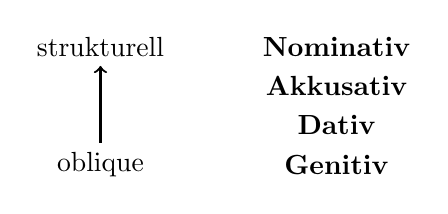
\begin{tikzpicture}
    \node (obl)                             {oblique};
    \node (gen) at ([shift={( 3,0)}]   obl) {\textbf{Genitiv}};
    \node (dat) at ([shift={( 0,0.5)}] gen) {\textbf{Dativ}};
    \node (akk) at ([shift={( 0,0.5)}] dat) {\textbf{Akkusativ}};
    \node (nom) at ([shift={( 0,0.5)}] akk) {\textbf{Nominativ}};
    \node (str) at ([shift={(-3,0)}]   nom) {strukturell};
    \draw [->, thick] (obl) to (str);
  \end{tikzpicture}
  \caption{Kasushierarchie}
  \label{fig:kashier}
\end{figure}

\index{Kasus!strukturell}
\index{Kasus!oblique}
Auf Basis dieser Überlegungen kommt man zu einer Hierarchie der Kasus bezüglich ihrer \textit{Strukturalität} bzw.\ \textit{Obliqueheit}.
Je prototypischer verbgebunden ein Kasus ist und je weniger semantisch oder funktional spezifisch er ist, desto weiter oben steht er in der Hierarchie bzw.\ desto \textit{struktureller} ist er.
Das Gegenteil von strukturell nennen wir \textit{oblique}.
Die Hierarchie wird in Abbildung~\ref{fig:kashier} dargestellt, Tabelle~\ref{tab:eigenschaftenderkasus} fasst wichtige Eigenschaften der Kasus zusammen.
In Tabelle~\ref{tab:eigenschaftenderkasus} ist mit \textit{eigene Semantik} gemeint, ob die Kasus, wenn sie von Verben abhängen, trotzdem eine eigene Semantik haben.%
\footnote{Neben den Beispielen weiter oben ist hierzu auch Abschnitt~\ref{sec:objekte} relevant.}
Die Auflistung der Kasus erfolgt in diesem Buch immer in der Reihenfolge der Obliqueheitshierarchie und nie in der schulgrammatischen Abfolge (Nominativ, Genitiv, Dativ, Akkusativ).
Bei der Darstellung der Pronomina und Adjektive wird sich diese Abfolge auch als sehr nützlich erweisen, weil dann die meisten synkretistischen Formen untereinanderstehen.

\begin{table}[!htbp]
  \begin{tabular}{lp{0.1cm}llll}
    \lsptoprule
     \textbf{Eigenschaft} && \textbf{Nominativ} & \textbf{Akkusativ} & \textbf{Dativ} & \textbf{Genitiv} \\
    \hline
    verbregiert && fast immer & oft & oft & selten \\
    eigene Semantik && nein & fast nie & manchmal & manchmal \\
    attributiv && nein & nein & nein & ja \\
    präpositionsregiert && nie & oft & oft & oft \\
    \lspbottomrule
  \end{tabular}
  \caption{Eigenschaften der Kasus}
  \label{tab:eigenschaftenderkasus}
\end{table}

Das Merkmal \textsc{Kasus} kommt also exklusiv bei Nomina vor und ist nur bei den obliquen Kasus und auch dort nur mit starken Einschränkungen semantisch motiviert.
Es liegt innerhalb von NPs immer Kongruenz bezüglich \textsc{Kasus} vor.
Die Werte des Merkmals \textsc{Kasus} sind prototypischerweise -- wenn auch nicht ausschließlich -- durch Rektion gesetzt.

\subsection{Person}

\label{sec:person}

\index{Person!Nomen}
\index{Pronomen!Personal--}
Das Merkmal \textsc{Person} (mit den Werten \textit{1}, \textit{2} und \textit{3}) ist ein eher semantisch und pragmatisch als strukturell motiviertes Merkmal.
Prototypische Träger des Merkmals \textsc{Person} sind die sogenannten \textit{Personalpronomina}.
Überlegen wir, was mit den Pronomina in (\ref{ex:flex9000}) kodiert wird, wobei jeweils Singular und Plural zusammengefasst werden und \textit{er}, \textit{sie} und \textit{es} von \textit{sie} vertreten werden.

\begin{exe}
  \ex \label{ex:flex9000}
  \begin{xlist}
    \ex{Ich unterstütze/Wir unterstützen den FCR Duisburg.}
    \ex{Du unterstützt/Ihr unterstützt den FCR Duisburg.}
    \ex{Sie/Diese/Jene/Eine/Man\ldots unterstützt den FCR Duisburg.}
    \ex{Sie/Diese/Jene/Einige/\ldots unterstützen den FCR Duisburg.}
  \end{xlist}
\end{exe}

\index{Deixis}
\index{Pronomen!deiktisch}

Zum Verständnis von Sätzen, die \textit{ich}, \textit{wir}, \textit{du} und \textit{ihr} enthalten, ist es erforderlich, die Sprechsituation des Satzes zu kennen.
Nur, wenn diese bekannt ist, kann erschlossen werden, wer oder was mit diesen Pronomina bezeichnet wird.
Sprecher \textit{verweisen} mit diesen Pronomina sozusagen auf bestimmte in der Sprechsituation anwesende Dinge, und man spricht von \textit{deiktischen} Ausdrücken gemäß Definition~\ref{def:deixis}.

\Definition{Deiktischer Ausdruck}{\label{def:deixis}%
\textit{Deiktische Ausdrücke} sind verweisende Ausdrücke, deren Bedeutung nur in einer Kommunikationssituation erschließbar ist.
}

Da mit deiktischen Ausdrücken auf die Kommunikationssituation Bezug genommen wird, kann man sagen, dass hier eine \textit{pragmatische} Motivation vorliegt.
Das Phänomen der Deixis findet man nicht nur bei Personenbezügen in der ersten oder zweiten Person, sondern typischerweise auch bei lokalen Ausdrücken (\textit{hier}, \textit{dort}) und temporalen Ausdrücken (\textit{heute}, \textit{jetzt}, \textit{nächste Woche}).

Die dritte Person ist insofern von der ersten und der zweiten verschieden, als prototypischerweise keine Kenntnis der Kommunikationssituation erforderlich ist, um ihre Bedeutung zu dekodieren.
Die kurzen Texte in (\ref{ex:flex4242})--(\ref{ex:flex4244}) zeigen dies.

\begin{exe}
  \ex{\label{ex:flex4242}Sarah backt ihrer Freundin einen Kuchen.\\
    Sie verwendet nur fair gehandelten unraffinierten Rohrzucker.}
  \ex{\label{ex:flex4243}Sarah backt ihrer Freundin einen Kuchen.\\
    Er besteht nur aus fair gehandelten Zutaten.}
  \ex{\label{ex:flex4244}Sarah backt ihrer Freundin einen Kuchen.\\
    Sie soll ihn zum Geburtstag geschenkt bekommen.}
\end{exe}

\index{Anapher}
\index{Pronomen!anaphorisch}

Die Pronomina nehmen jeweils die Bedeutung einer im Text vorausgehenden NP wieder auf.
In (\ref{ex:flex4242}) bezeichnet \textit{sie} dieselbe Person wie \textit{Sarah} im vorausgehenden Satz usw.
Solche Pronomina nennt man \textit{anaphorische Pronomina} oder allgemein \textit{Anaphern} gemäß Definition~\ref{def:anaphern}.

\Definition{Anapher, Antezedens, Korreferenz}{\label{def:anaphern}%
\textit{Anaphern} sind Ausdrücke, die die Bedeutung eines im Satz oder Text vorangehenden Ausdrucks (des \textit{Antezedens}) wieder aufnehmen.
Anapher und Antezedens sind \textit{korreferent} (Gleiches bezeichnend).
\index{Antezedens}\index{Korreferenz}
}

Dass es keine eindeutigen grammatischen Kriterien zur Bestimmung des Antezedens einer Anapher gibt, sieht man an den Beispielen (\ref{ex:flex4242}) und (\ref{ex:flex4244}).
Das Pronomen \textit{sie} ist hier offensichtlich einmal korreferent mit \textit{Sarah} und einmal mit \textit{ihrer Freundin}.
Dass dies so ist, erkennen wir eindeutig an der Gesamtbedeutung der Sätze, nicht etwa an einer Übereinstimmung von Kasus:
Hier steht das Antezedens im Nominativ und die Anapher im Dativ.
Die mögliche Korreferenz von nominalen Anaphern wird allerdings durch \textsc{Numerus} und \textsc{Genus} eingeschränkt, die bei der Anapher im Normalfall mit dem Antezedens übereinstimmen müssen.

Korreferenz wird mit numerischen \textit{Indizes} (Singular \textit{Index}) notiert, also tiefgestellten Nummern nach der entsprechenden NP, die ggf.\ eingeklammert werden muss, um anzuzeigen, dass es eine Konstituente aus mehreren Wörtern ist.\index{Index}
Wir wiederholen hier die Sätze (\ref{ex:flex4242})--(\ref{ex:flex4244}) als (\ref{ex:flex-4242-r})--(\ref{ex:flex-4244-r}) und setzen die Indizes.

\begin{exe}
  \ex{\label{ex:flex-4242-r}Sarah$_{\textnormal{1}}$ backt [ihrer Freundin]$_{\textnormal{2}}$ [einen Kuchen]$_{\textnormal{3}}$.\\
    Sie$_{\textnormal{1}}$ verwendet nur fair gehandelten unraffinierten Rohrzucker.}
  \ex{\label{ex:flex-4243-r}Sarah$_{\textnormal{1}}$ backt [ihrer Freundin]$_{\textnormal{2}}$ [einen Kuchen]$_{\textnormal{3}}$.\\
    Er$_{\textnormal{3}}$ besteht nur aus fair gehandelten Zutaten.}
  \ex{\label{ex:flex-4244-r}Sarah$_{\textnormal{1}}$ backt [ihrer Freundin]$_{\textnormal{2}}$ [einen Kuchen]$_{\textnormal{3}}$.\\
    Sie$_{\textnormal{2}}$ soll ihn$_{\textnormal{3}}$ zum Geburtstag geschenkt bekommen.}
\end{exe}

Zwei Ausdrücke mit demselben Index sind korreferent und werden manchmal auch \textit{koindiziert} genannt.
Unabhängig davon, welche Zahl man als Index wählt, werden zwei Ausdrücke mit der gleichen Index-Ziffer immer so gelesen, dass sie die gleiche Bedeutung haben.
Mit Bedeutung ist hier gemeint, dass sie auf dieselben Gegenstände (ob abstrakt oder konkret) in der Welt verweisen, bzw. dass sie dieselben Gegenstände bezeichnen.
In (\ref{ex:flex-4242-r}) verweisen \textit{Sarah} und \textit{sie} auf dasselbe Objekt bzw.\ dieselbe Person.

Die dritte Person ist allerdings nicht immer, sondern nur bei den Personalpronomina typisch anaphorisch.
Die Kongruenz mit dem Verb zeigt, dass alle gewöhnlichen Substantive und im Grunde alle Pronomina außer den Personalpronomen der ersten und zweiten Person auch statisch [\textsc{Person}: \textit{3}] sind, s.\ (\ref{ex:flex6263}).

\begin{exe}
  \ex \label{ex:flex6263}
  \begin{xlist}
    \ex{Ich geh-e.}
    \ex{Du geh-st.}
    \ex{Er/sie/es/die Trainerin/Martina/diese geh-t.}
  \end{xlist}
\end{exe}

Auch die Pronomina der dritten Person, die typisch anaphorisch sind, haben manchmal eine deiktische Lesart, die unter Umständen durch Hinzufügung von Adverben wie \textit{hier} oder \textit{dort} noch verstärkt wird.

\begin{exe}
  \ex{Er hier hat noch kein Ticket.}
  \ex{Jene dort ist die Fußballerin des Jahres.}
\end{exe}

\subsection{Genus}

\index{Genus}

\textsc{Genus} ist das definierende statische Merkmal der Substantive (s.\ Abschnitt~\ref{sec:verbennominawortklassen}).
Die Betrachtung einiger Beispiele zeigt, dass \textsc{Genus} keine semantische Funktion hat, (\ref{ex:flex8881}).

\begin{exe}
  \ex \label{ex:flex8881}
  \begin{xlist}
    \ex{Die Petunie ist eine Blume.}
    \ex{Der Enzian ist eine Blume.}
    \ex{Das Veilchen ist eine Blume.}
  \end{xlist}
\end{exe}

Das unterschiedliche \textsc{Genus}-Merkmal der Substantive in (\ref{ex:flex8881}) hat zur Folge, dass der Artikel (und ggf.\ auch hinzutretende Adjektive) mit einem kongruierenden \textsc{Genus}-Merkmal auftreten.
Die strukturelle Bedeutung des Genus ist also auf die NP beschränkt.
Darüber hinaus haben Genusunterschiede keinerlei Effekt auf den Satzbau, es gibt \zB keine \textsc{Genus}-Kongruenz beim Verb.
 An den Beispielen in (\ref{ex:flex8881}) ist auch gut erkennbar, dass Genus nicht semantisch motiviert ist.
Petunien, Enzian und Veilchen haben nichts \textit{Weibliches}, \textit{Männliches} und \textit{Sächliches} an sich, wie die terminologisch schlechten deutschen Übersetzungen von \textit{Femininum}, \textit{Maskulinum} und \textit{Neutrum} suggerieren.%
\footnote{Strenggenommen bedeutet lateinisch \textit{ne-utrum} ungefähr \textit{weder noch}.}
Alle drei können als \textit{Blume} (feminin) bezeichnet werden, ohne dass dies besonders auffallen würde.
Lediglich bei Personenbezeichnungen (und eingeschränkt Tierbezeichnungen) gibt es eine überwiegende Übereinstimmung von biologischem Geschlecht und \textsc{Genus}.

\textsc{Genus} ist also ein Merkmal, über das in syntaktischen Strukturen Beziehungen hergestellt werden (\textsc{Genus}-Kongruenz in der nominalen Gruppe), aber es ist in keiner Weise besonders motiviert.
Die drei Genera leisten lediglich eine lexikalische Unterklassifikation der Substantive.
Da sie relevante Unterschiede im Flexionsverhalten mit sich bringen, wird \textsc{Genus} in den Abschnitten~\ref{sec:subst} sowie~\ref{sec:artikelpronomen} und~\ref{sec:adjektive} weiterhin eine wichtige Rolle spielen.


\subsection{Die nominalen Merkmale im Überblick}

Wir deklarieren jetzt abschließend die Merkmale, die im Wesentlichen alle Nomina haben und fassen die wichtigen Ergebnisse zusammen.
Die Bezeichnungen der Merkmale und Werte werden im weiteren Verlauf ggf.\ transparent abgekürzt (\textsc{Numerus} zu \textsc{Num}, \textit{singular} zu \textit{sg} usw.).

\begin{exe}
  \ex{\textsc{Numerus}: \textit{singular}, \textit{plural}}
  \ex{\textsc{Kasus}: \textit{nominativ}, \textit{akkusativ}, \textit{dativ}, \textit{genitiv}}
  \ex{\textsc{Person}: \textit{1}, \textit{2}, \textit{3}}
  \ex{\textsc{Genus}: \textit{maskulin}, \textit{neutral}, \textit{feminin}}
\end{exe}

\textsc{Numerus} ist semantisch motiviert (Anzahl der bezeichneten Dinge), \textsc{Kasus} ist überwiegend strukturell motiviert (Rektion durch Verben und Präpositionen), \textsc{Person} ist wiederum semantisch bzw.\ pragmatisch motiviert (Deixis und Anaphorik), und \textsc{Genus} kann bis auf wenige Ausnahmen als nicht motiviert gelten.
Statisch ist \textsc{Genus} beim Substantiv sowie \textsc{Person} bei allen Pronomina und Substantiven.
Innerhalb einer nominalen Gruppe (typischerweise bestehend aus Artikel, ggf.\ Adjektiven und dem Substantiv) kongruieren alle Nomina in \textsc{Numerus}, \textsc{Kasus} und \textsc{Genus}.
Das nominale Subjekt (vgl.\ Abschnitt~\ref{sec:subjekt}) kongruiert mit dem Verb in \textsc{Numerus} und \textsc{Person}.
Der Rest dieses Kapitels ist jetzt der Frage gewidmet, durch welche formalen Mittel diese Merkmale eindeutig oder nicht eindeutig an den Nomina markiert werden.


\Zusammenfassung{%
  Die verschiedenen nominalen Kategorien (bzw.\ Merkmale) sind teilweise semantisch\slash pragmatisch motiviert, teilweise aber eher strukturell bzw.\ rein grammatisch.
  Kasus lassen sich in einer Hierarchie anordnen, je nachdem wie stark sie einen eigenständigen semantischen Beitrag leisten (oblique) bzw.\ nur Rektionsanforderungen erfüllen (strukturell).
}


\section{Substantive}

\label{sec:subst}

In diesem Abschnitt geht es darum, wie die verschiedenen \textsc{Kasus}"=\textsc{Numerus}"=Formen der Substantive formal gebildet werden, und zwar in Abhängigkeit von ihrer Flexionsklasse, die wiederum stark durch das statische \textsc{Genus}"=Merkmal vorbestimmt wird.
Wie eindeutig die Form (\zB in Form eines Suffixes) dabei tatsächlich \textsc{Kasus} und \textsc{Numerus} als Markierungsfunktion hat, wird für die einzelnen Flexionsklassen ebenfalls untersucht.%
\footnote{Im weiteren Verlauf des Kapitels wird überwiegend vereinfacht von \textit{Kasus}, \textit{Numerus}, \textit{Nominativ}, \textit{Plural} usw. gesprochen, ohne die genauen Merkmalsangaben wie [\textsc{Kasus}: \textit{nom}] usw. zu liefern.
Die Merkmalsnotation wird benutzt, wenn die formale Notation für die Argumentation wichtig ist.}

\subsection{Traditionelle Flexionsklassen}

\label{sec:nominaflexionsklassen}
\label{Substantiv!Flexion}

\begin{figure}[!htbp]
    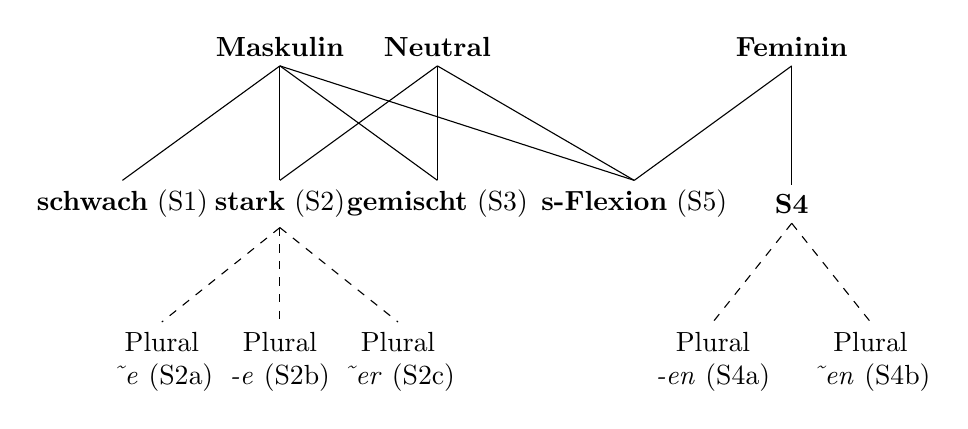
\begin{tikzpicture}[every text node part/.style={align=center}]
      \node (MaskN)    at (2,4)   {\textbf{Maskulin}};
      \node (NeutN)    at (4,4)   {\textbf{Neutral}};
      \node (FemN)     at (8.5,4) {\textbf{Feminin}};

      \node (schwachN) at (0,2)   {\textbf{schwach} (S1)};
      \node (starkN)   at (2,2)   {\textbf{stark} (S2)};
      \node (gemistN)  at (4,2)   {\textbf{gemischt} (S3)};
      \node (sFlexN)   at (6.5,2) {\textbf{s-Flexion} (S5)};
      \node (s4N)      at (8.5,2) {\textbf{S4}};

      \node (EPlu)     at (0.5,0) {Plural\\\textit{\char`~e} (S2a)};
      \node (ePlu)     at (2,0)   {Plural\\\textit{-e} (S2b)};
      \node (erPlu)    at (3.5,0) {Plural\\\textit{\char`~er} (S2c)};

      \node (enPlu)    at (7.5,0) {Plural\\\textit{-en} (S4a)};
      \node (EnPlu)    at (9.5,0) {Plural\\\textit{\char`~en} (S4b)};

      \draw (MaskN.south)  -- (schwachN.north);
      \draw (MaskN.south)  -- (starkN.north);
      \draw (MaskN.south)  -- (gemistN.north);
      \draw (MaskN.south)  -- (sFlexN.north);

      \draw (NeutN.south)  -- (starkN.north);
      \draw (NeutN.south)  -- (gemistN.north);
      \draw (NeutN.south)  -- (sFlexN.north);

      \draw (FemN.south)   -- (s4N.north);
      \draw (FemN.south)   -- (sFlexN.north);

      \draw [dashed] (starkN.south) -- (EPlu.north);
      \draw [dashed] (starkN.south) -- (ePlu.north);
      \draw [dashed] (starkN.south) -- (erPlu.north);

      \draw [dashed] (s4N.south)    -- (enPlu.north);
      \draw [dashed] (s4N.south)    -- (EnPlu.north);
    \end{tikzpicture}
  \caption{Traditionelle Flexionsklassen der Substantive}
  \label{fig:substflexklassen}
\end{figure}

Die traditionellen Flexionsklassen teilen die Substantive zunächst nach Genus und dann innerhalb des Maskulinums und Neutrums weiter nach der sogenannten \textit{Stärke} (\textit{stark}, \textit{schwach}, \textit{gemischt}).
Zusätzlich gibt es eine Klasse, die wir hier \textit{s-Flexion} nennen, und in die Substantive aus allen Genera fallen.
Abbildung~\ref{fig:substflexklassen} zeigt die Zusammenhänge, wobei die gestrichelten Linien Subklassifizierungen unterhalb des traditionellen terminologischen Rasters andeuten.
Einen Überblick über die wichtigen Flexionsmuster mit Beispielen gibt Tabelle~\ref{tab:tradflexsubst}.
In Tabelle~\ref{tab:tradflexsubst} ist der Typ S2b (\textit{Gurt}, \textit{Schaf}) nicht extra aufgeführt, weil er sich von S2a (\textit{Stuhl}, \textit{Floß}) nur durch das Fehlen des Umlauts im Plural unterscheidet.
Innerhalb der Genera sind die Endungen nicht gleichberechtigt.
Die meisten Feminina bilden den Plural mit \textit{-en}, die meisten Maskulina und Neutra mit \textit{-e}.
Während der Umlaut für das Femininum bei \textit{\char`~e} obligatorisch ist, ist er es bei \textit{-e} bzw.\ \textit{\char`~e} im Maskulinum und Neutrum nicht.

\index{Substantiv!Stärke}
\index{Substantiv!Subklassen}

\begin{table}[!htbp]
  \resizebox{\textwidth}{!}{
    \begin{tabular}{llp{0mm}lp{2mm}llp{1mm}lp{2mm}llp{2mm}l}
      \lsptoprule
      \multicolumn{2}{c}{} && \multicolumn{1}{l}{\textbf{Maskulinum}} && \multicolumn{4}{l}{\textbf{Maskulinum und Neutrum}} && \multicolumn{2}{l}{\textbf{Femininum}} && \multicolumn{1}{l}{\textbf{s-Flexion}} \\
      \multicolumn{2}{c}{} && \multicolumn{1}{l}{\textbf{schwach (S1)}} && \multicolumn{2}{l}{\textbf{stark (S2)}} && \multicolumn{1}{l}{\textbf{gemischt (S3)}} && \multicolumn{2}{l}{\textbf{(S4)}} && \multicolumn{1}{l}{\textbf{(S5)}} \\
      \midrule
      \multirow{4}{*}{\textbf{Sg}} & \textbf{Nom} && Mensch && Stuhl & Haus && Staat && Frau & \multicolumn{1}{l}{Sau} && Auto \\
      & \textbf{Akk} && Mensch-en && Stuhl & Haus && Staat && Frau & \multicolumn{1}{l}{Sau} && Auto \\
      & \textbf{Dat} && Mensch-en && Stuhl & Haus && Staat && Frau & \multicolumn{1}{l}{Sau} && Auto \\
      & \textbf{Gen} && Mensch-en && Stuhl-es & Haus-es && Staat-(e)s && Frau & \multicolumn{1}{l}{Sau} && Auto-s \\
      \midrule
      \multirow{4}{*}{\textbf{Pl}} & \textbf{Nom} && Mensch-en && Stühl-e & Häus-er && Staat-en && Frau-en & \multicolumn{1}{l}{Säu-e} && Auto-s \\
      & \textbf{Akk} && Mensch-en && Stühl-e & Häus-er && Staat-en && Frau-en & \multicolumn{1}{l}{Säu-e} && Auto-s \\
      & \textbf{Dat} && Mensch-en && Stühl-en & Häus-ern && Staat-en && Frau-en & \multicolumn{1}{l}{Säu-en} && Auto-s \\
      & \textbf{Gen} && Mensch-en && Stühl-e & Häus-er && Staat-en && Frau-en & \multicolumn{1}{l}{Säu-e} && Auto-s \\
      \lspbottomrule
    \end{tabular}
  }
  \caption{Traditionelle Flexionsklassen der Substantive}
  \label{tab:tradflexsubst}
\end{table}

Die Unterscheidung nach Stärke betrifft nur die Maskulina und Neutra, dabei aber nicht die s-Flexion.
Es reicht im Prinzip die Kenntnis des Genus sowie die Form des Genitiv Singular und des Nominativ Plural, um die traditionelle Flexionsklasse eines Substantivs zu bestimmen.
Der Entscheidungsbaum in Abbildung~\ref{fig:substklassentsch} zeigt, wie die primäre Flexionsklasse eines Substantivs ermittelt werden kann, wenn man die Formen beherrscht.
Als diagnostische Form wird für die Unterscheidung von starken und gemischten Substantiven der Nominativ Plural gewählt.
Da der Akkusativ Plural und der Genitiv Plural gleichlautend mit dem Nominativ Plural sind, könnte man hier genausogut eine dieser beiden Formen nehmen.
Zusammengefasst lässt sich aus Abbildung~\ref{fig:substklassentsch} als Faustregel für die Unterscheidung nach Stärke wie in (\ref{ex:wuppdich1}) und (\ref{ex:wuppdich2}) formulieren.

\begin{figure}[!htbp]
  \centering
  \begin{forest}
    for tree={l sep=2em},
    decide/.style={draw, chamfered rectangle, inner sep=2pt},
    finall/.style={rounded corners, fill=gray}
      [Genus?, s sep=10em, decide
        [Genitiv\\Singular?, s sep+=2em, decide,
          edge label={node[pos=0.6, above, sloped, font=\scriptsize]{maskulin\slash neutrum}}
          [\whyte{Schwache}\\\whyte{Maskulina (S1)}, finall,
            edge label={node[pos=0.7, above, sloped, font=\scriptsize]{-(e)n}}
          ]
          [Nominativ\\Plural?, s sep+=0.5em, decide,
            edge label={node[pos=0.7, above, sloped, font=\scriptsize]{-(e)s}}
            [\whyte{Gemischte Maskulina}\\\whyte{und Neutra (S3)}, finall,
              edge label={node[pos=0.7, above, sloped, font=\scriptsize]{-(e)n}}]
            [\whyte{Starke Maskulina}\\\whyte{und Neutra (S2)}, finall,
              edge label={node[pos=0.7, above, sloped, font=\scriptsize]{\char`~er\slash \char`~e\slash-e}}]
          ]
        ]
        [\whyte{Feminina (S4)}, finall,
          edge label={node[midway, above, sloped, font=\scriptsize]{feminin}}]
      ]
  \end{forest}
  \caption{Entscheidungsbaum für die Flexionsklassenzugehörigkeit}
  \label{fig:substklassentsch}
\end{figure}

\begin{exe}
  \ex\label{ex:wuppdich1} Maskulinum\\
    Genitiv Singular \textit{-en}: schwach
  \ex\label{ex:wuppdich2} Maskulinum\slash Neutrum
  \begin{xlist}
    \ex\label{ex:wuppdich2a} Genitiv Singular \textit{-es}, Nominativ Plural \textit{\char`~e}/\textit{-e}/\textit{\char`~er}: stark
    \ex\label{ex:wuppdich2b} Genitiv Singular \textit{-es}, Nominativ Plural \textit{-en}: gemischt
  \end{xlist}
\end{exe}

In dieser etwas unübersichtlichen Darstellung gibt es also die fünf eigenständigen Flexionsmuster S1--S5, bei Zählung der Unterklassen S2a--S2c, S4a und S4b sogar acht.
Im Folgenden soll diese scheinbar starke Differenzierung auf das Wesentliche reduziert werden.
Dazu fragen wir zunächst, wie Numerus markiert wird (Abschnitt~\ref{sec:pluralmark}).
Getrennt davon fragen wir, wie Kasus markiert wird (Abschnitt~\ref{sec:kasusmark}).
Dann folgt eine kurze Diskussion der besonderen Kasus"=Numerus"=Markierungen bei den schwachen Substantiven (Abschnitt~\ref{sec:schwachsubst}).
Schließlich wird alles in Abschnitt~\ref{sec:neuenklassen} in einem vereinfachten Klassensystem zusammengefasst.


\subsection{Numerusflexion}

\label{sec:pluralmark}
\index{Substantiv!Numerusflexion}
\index{Substantiv!Plural}

\begin{table}[!htbp]
  \centering
  \begin{tabular}{llll}
    \lsptoprule
    \textbf{Klasse} & \textbf{Kasus} & \textbf{Sg} & \textbf{Pl} \\
    \midrule
    S1 & Nom & (der) Mensch & (die) Mensch-en \\
    S2a & Gen & (des) Stuhl-es & (der) Stühl-e \\
    S2b & Akk & (den) Gurt & (die) Gurt-e \\
    S2c & Dat & (dem) Haus & (den) Häus-ern \\
    S3 & Akk & (den) Staat & (die) Staat-en \\
    S4a & Nom & (die) Frau & (die) Frau-en \\
    S4b & Nom & (die) Sau & (die) Säu-e \\
    \midrule
    S1 & Akk & (den) Mensch-en & (die) Mensch-en \\
    S5 & Gen & (des) Auto-s & (der) Auto-s \\
    \lspbottomrule
  \end{tabular}
  \caption{Beispiele für die Pluralmarkierung beim Substantiv}
  \label{tab:sgplvergl}
\end{table}

Wenn wir Kasusformen gleicher Wörter in Singular und Plural vergleichen, ist die Plural-Form fast immer von der Singular-Form unterscheidbar, wofür einige Beispiele in Tabelle~\ref{tab:sgplvergl} gesammelt wurden.
Die einzigen Ausnahmen bilden der Akkusativ, Dativ und Genitiv der schwachen Maskulina (S1) und der Genitiv der Maskulina und Neutra der s-Flexion (S5), bei denen die Formen des Singulars und des Plurals identisch sind.
Auch diese Fälle sind in Tabelle~\ref{tab:sgplvergl} bebeispielt.
Eine schwächere Formulierung wäre:
Der Plural ist immer gleich stark markiert wie oder stärker markiert als der Singular.

Allein die Tatsache, dass der Plural gegenüber dem Singular i.\,d.\,R.\ gekennzeichnet ist, ist ein Indiz dafür, dass die vorkommenden Affixe \textsc{Numerus} als Markierungsfunktion haben.
Hinzu kommt, dass der Plural innerhalb jedes Flexionstyps durch ein einheitliches Element gekennzeichnet ist.
Diese einheitlichen Elemente sind in Tabelle~\ref{tab:plaffixe} zusammengefasst.
Es fällt auf, dass bei allen Flexionsklassen außer den schwachen das Affix eindeutig dem Plural zugeordnet werden kann.%
\footnote{Bei Genitiven wie \textit{des Auto-s} und \textit{der Auto-s} ist die Zuordnung des \textit{-s} zum Plural zugegebenermaßen nicht ganz eindeutig zwingend, aber dennoch möglich und aus der Betrachtung des Gesamtsystems heraus naheliegend.}
Die schwachen Substantive (S1) bilden eine Ausnahme und sollen erst später als solche betrachtet werden (Abschnitt~\ref{sec:schwachsubst}).
Bei den schwachen Substantiven kommt dasselbe Affix \textit{-en} auch in allen Formen des Singulars außer im Nominativ vor.
Der Vergleich dieser Tabelle mit Tabelle~\ref{tab:tradflexsubst} zeigt die Einheitlichkeit der Pluralmarkierung in allen Klassen.

\begin{table}[!htbp]
  \centering
  \resizebox{\textwidth}{!}{
    \begin{tabular}{lp{0mm}lp{1mm}lllp{1mm}lp{1mm}llp{1mm}l}
      \lsptoprule
      \textbf{Klasse} && Mask schwach && \multicolumn{3}{l}{Mask\slash Neut stark} && Mask\slash Neut gem. && \multicolumn{2}{l}{Fem} && s-Flexion \\
      \textbf{Nummer} && S1 && S2a & S2b & S2c && S3 && S4a & S4b && S5 \\
      \midrule
      \textbf{Markierung} && \textbf{-en} && \textbf{\char`~e} & \textbf{-e} & \textbf{\char`~er} && \textbf{-en} && \textbf{-en} & \textbf{\char`~e} && \textbf{-s} \\
      \textbf{Beispiel} && Mensch-en && Stühl-e & Gurt-e & Häus-er && Staat-en && Frau-en & Säu-e && Auto-s \\
      \lspbottomrule
    \end{tabular}
  }
  \caption{Übersicht über die Plural-Affixe mit Beispielen}
  \label{tab:plaffixe}
\end{table}

Es handelt sich in allen Fällen um Bildungen mittels Affixen.
Wie bereits erwähnt ist die prototypische (und häufigste) Pluralbildung bei den Maskulina und Neutra die auf \textit{\char`~e} (seltener ohne Umlaut \textit{-e}) und bei den Feminina die auf \textit{-en}.
Einige weitere scheinbare Untertypen der Pluralbildung ergeben sich, wenn Pluralbildungen wie in Tabelle~\ref{tab:schwaimplural} hinzugezogen werden.
Diese Fälle sind bisher (vor allem in Tabelle~\ref{tab:tradflexsubst}) noch nicht erwähnt worden.
Die schwachen Substantive sollen wieder zunächst ignoriert werden.

\begin{table}[!htbp]
  \centering
  \resizebox{\textwidth}{!}{
    \begin{tabular}{llp{1mm}llp{1mm}llp{1mm}ll}
      \lsptoprule
      \multicolumn{2}{l}{\textbf{schwach}} && \multicolumn{2}{l}{\textbf{gemischt}} && \multicolumn{2}{l}{\textbf{Fem S4a}} && \multicolumn{2}{l}{\textbf{Fem S4b}}\\
      \textbf{voll} & \textbf{reduziert} && \textbf{voll} & \textbf{reduziert} && \textbf{voll} & \textbf{reduziert} && \textbf{voll} & \textbf{reduziert} \\
      \midrule
      Mensch-en & Löwe-n && Staat-en & Ende-n && Frau-en & Nudel-n && Säu-e & Mütter-$\emptyset$ \\
      \lspbottomrule
    \end{tabular}
  }
  \caption{Volle und um Schwa reduzierte Plural-Affixe}
  \label{tab:schwaimplural}
\end{table}

\index{Schwa!Tilgung}
Diese vermeintlichen Ausnahmen oder Unterklassen sind nicht zufällig verteilt und können nach einer einfachen Regel vorhergesagt werden.
Das Plural-Affix ist bei \textit{Löwe}, \textit{Ende} und \textit{Nudel} jeweils nicht \textit{-en}, sondern \textit{-n}.
Bei \textit{Mütter} tritt zwar der Umlaut ein, aber die Endung \textit{\char`~e} wird nicht suffigiert.
Hinzu kommen noch Wörter wie \textit{Läufer}, die in die Tabellen nicht aufgenommen wurden, die gar kein Pluralkennzeichen zu haben scheinen.
Man kann in diesen Fällen davon ausgehen, dass das Schwa des Suffixes (also \textit{-e} mit oder ohne Umlaut bzw.\ \textit{-en}) jeweils aus phonotaktischen Gründen ausfällt, nämlich um Doppelungen von Schwa bzw.\ Schwa-Silben zu vermeiden.
Die Formen mit direkter Abfolge von zwei Schwas \textit{\Ast Löwe-en} und \textit{\Ast Ende-en} sind im Deutschen phonotaktisch gänzlich ausgeschlossen.
\textit{\Ast Nudel-en}, \textit{\Ast Mütter-e} oder \textit{\Ast Läufer-e} wären im Prinzip phonotaktisch möglich (vgl.\ \textit{ich buttere}).
Allerdings bilden die Plurale der einfachen Substantive prototypisch einen trochäischen (also zweisilbigen) Fuß.
Deshalb wird bei femininen Substantiven, die auf \textit{el}, \textit{er} und \textit{en} enden, ebenfalls das phonologisch schwache Schwa des Plural-Affixes getilgt.
Alle Formen des Paradigmas behalten also eine einheitliche Fußform.
Als Besonderheit bleibt dann in der Klasse von \textit{Mutter} nur der Umlaut als sichtbares Pluralkennzeichen, und bei \textit{Läufer} ist der Plural gar nicht formal erkennbar, weil der Umlaut bereits im Singularstamm vorliegt.
Satz~\ref{satz:schwainflexionssuffixen} fasst schließlich das Phänomen zusammen.


\Satz{Schwa-Tilgung in Flexionssuffixen}{\label{satz:schwainflexionssuffixen}%
Geht der Stamm eines Substantivs auf \textit{e} oder auf \textit{el}, \textit{er}, \textit{en} aus, wird das Schwa in antretenden Flexionsaffixen getilgt.
Ein Affix der Form \textit{\char`~e} löst dabei Umlaut aus, auch wenn es selbst vollständig getilgt wird.
}

Das System der Plural-Markierung ist also insofern relativ klar, als es für jede Flexionsklasse ein eindeutiges Plural-Kennzeichen gibt.
Die Affixe in Tabelle~\ref{tab:plaffixe} (evtl. mit Ausnahme des \textit{-en} bei den schwachen) haben die Markierungsfunktion, [\textsc{Numerus}: \textit{pl}] anzuzeigen.

\subsection{Kasusflexion}

\label{sec:kasusmark}
\index{Substantiv!Kasusflexion}

Wenn wir jetzt Tabelle~\ref{tab:tradflexsubst} als Tabelle~\ref{tab:tradflexsubst-r} wiederholen und die Plural-Affixe vom restlichen Material abtrennen, wird schnell klar, dass das verbleibende Affix-Material eine äußerst sparsame Markierung von Kasus darstellt.
Zusätzlich wurden die seltenen archaischen Dative auf \textit{-e} bei den starken und gemischten Substantiven aufgenommen.

\begin{table}[!htbp]
  \centering
  \resizebox{\textwidth}{!}{
    \begin{tabular}{llp{0mm}lp{2mm}llp{1mm}lp{2mm}llp{2mm}l}
      \lsptoprule
      \multicolumn{2}{c}{} && \multicolumn{1}{l}{\textbf{Maskulinum}} && \multicolumn{4}{l}{\textbf{Maskulinum und Neutrum}} && \multicolumn{2}{l}{\textbf{Femininum}} && \multicolumn{1}{l}{\textbf{s-Flexion}} \\
      \multicolumn{2}{c}{} && \multicolumn{1}{l}{\textbf{schwach (S1)}} && \multicolumn{2}{l}{\textbf{stark (S2)}} && \multicolumn{1}{l}{\textbf{gemischt (S3)}} && \multicolumn{2}{l}{\textbf{(S4)}} && \multicolumn{1}{l}{\textbf{(S5)}} \\
      \midrule
      \multirow{4}{*}{\textbf{Sg}} & \textbf{Nom} && Mensch && Stuhl & Haus && Staat && Frau & \multicolumn{1}{l}{Sau} && Auto \\
      & \textbf{Akk} && Mensch-en && Stuhl & Haus && Staat && Frau & \multicolumn{1}{l}{Sau} && Auto \\
      & \textbf{Dat} && Mensch-en && Stuhl(-e) & Haus(-e) && Staat(-e) && Frau & \multicolumn{1}{l}{Sau} && Auto \\
      & \textbf{Gen} && Mensch-en && Stuhl-(e)s & Haus-(e)s && Staat-(e)s && Frau & \multicolumn{1}{l}{Sau} && Auto-s \\
      \midrule
      \multirow{4}{*}{\textbf{Pl}} & \textbf{Nom} && Mensch-en && Stühl-e & Häus-er && Staat-en && Frau-en & \multicolumn{1}{l}{Säu-e} && Auto-s \\
      & \textbf{Akk} && Mensch-en && Stühl-e & Häus-er && Staat-en && Frau-en & \multicolumn{1}{l}{Säu-e} && Auto-s \\
      & \textbf{Dat} && Mensch-en && Stühl-e-n & Häus-er-n && Staat-en && Frau-en & \multicolumn{1}{l}{Säu-e-n} && Auto-s \\
      & \textbf{Gen} && Mensch-en && Stühl-e & Häus-er && Staat-en && Frau-en & \multicolumn{1}{l}{Säu-e} && Auto-s \\
      \lspbottomrule
    \end{tabular}
  }
  \caption{Substantive mit Plural und potentiellen Kasus-Affixen}
  \label{tab:tradflexsubst-r}
\end{table}

An Tabelle~\ref{tab:tradflexsubst-r} ist sofort zu erkennen, welche Kasus beim Substantiv überhaupt markiert werden, zumindest wenn wir die schwachen Substantive außer Acht lassen.
Es gibt ausschließlich Markierungen für den Genitiv Singular (\textit{-es}) und den Dativ Plural (\textit{-n}), selten und archaisch auch für den Dativ Singular (\textit{-e}).
Im Dativ Plural wird immer \textit{-n} suffigiert, außer das Plural-Affix geht seinerseits bereits auf \textit{n} aus, oder es würden phonotaktisch schlechte Formen entstehen.
Formen wie \textit{\Ast Staat-en-n} und \textit{\Ast Auto-s-n} sind phonotaktisch im Deutschen inakzeptabel.

\index{Genitiv}\index{Dativ}
Im Genitiv Singular wird also außer bei den Feminina immer \textit{-es} suffigiert.
Die Unmarkiertheit des Genitiv Singular der Feminina betrifft auch die s-Flexion, \zB \textit{die Kekse der Oma}.
Ob in den sonstigen Formen Schwa (\textit{-es}) steht oder nicht steht (\textit{-s}), ist wie schon im Plural bei \textit{-en} und \textit{-n} auf Basis der Phonotaktik zu entscheiden.
Diese Alternation wurde in Vertiefung~\ref{vert:morphemeallomorphe} (vor allem Abbildung~\ref{fig:kondgensg} auf S.~\pageref{fig:kondgensg}) bereits beschrieben.
Geht der Stamm auf \textit{el}, \textit{er} oder \textit{en} aus, muss \textit{-s} stehen, \zB \textit{Mündel-s} und \textit{Eimer-s} (und nicht \textit{\Ast Mündel-es} und \textit{\Ast Eimer-es}).
In den meisten anderen Fällen ist das Schwa im Suffix optional, es geht also sowohl \textit{Stück-es} als auch \textit{Stück-s}.
Eine parallele Regularität gilt für den Dativ Singular auf \textit{-e} (\textit{dem Stück-e} oder \textit{dem Stück}), mit dem Unterschied, dass das Auftreten des Suffixes im Dativ generell sehr selten und stilistisch auffällig ist.
Satz~\ref{satz:kasusmarkierungsubst} fasst zusammen.


\index{Schwa!Tilgung}
\Satz{Kasusmarkierung beim Substantiv (außer schwach)}{\label{satz:kasusmarkierungsubst}%
Nur die obliquen Kasus Dativ und Genitiv werden überhaupt durch Affixe markiert.
Die strukturellen Kasus Nominativ und Akkusativ lauten typischerweise gleich und sind affixlos.
Der Dativ Plural wird einheitlich mit \textit{-n} markiert, der Genitiv Singular bei allen Substantiven außer den Feminina mit \textit{-es}.
}


Die Schwa-Haltigkeit des Affixes entscheidet sich wie schon im Plural anhand einer einfachen phonotaktischen Regel.
Die größte Attraktion im System bilden aber die schwachen Maskulina, zu denen jetzt (Abschnitt~\ref{sec:schwachsubst}) noch mehr gesagt wird.


\begin{Vertiefung}{Eigennamen und s-Flexion}
\index{Eigenname}

\noindent Bei der s-Flexion, besonders auffällig aber bei Verwandschaftsbezeichnungen wie \textit{Oma} und \textit{Opa}, ist die Flexionsklassenzugehörigkeit differenziert zu betrachten.
Die Beispiele in (\ref{ex:flex7289}) und (\ref{ex:flex7290}) illustrieren dies.


\begin{exe}
  \ex\label{ex:flex7289}
  \begin{xlist}
    \ex\label{ex:flex7289a} Das Haus der Oma von Mats erinnert ihn an seine Kindheit.
    \ex\label{ex:flex7289b} Die Oma-s von Mats konnten einander nicht ausstehen.
    \ex\label{ex:flex7289c} Oma-s Haus erinnert mich an meine Kindheit.
  \end{xlist}
  \ex\label{ex:flex7290}
  \begin{xlist}
    \ex\label{ex:flex7290a} Das Haus des Opa-s von Mats erinnert ihn an seine Kindheit.
    \ex\label{ex:flex7290b} Die Opa-s von Mats konnten einander nicht ausstehen.
    \ex\label{ex:flex7290c} Opa-s Haus erinnert mich an meine Kindheit.
  \end{xlist}
\end{exe}

Die jeweiligen Beispiele in (a) und (b) entsprechen den bisher gefundenen Regeln.
In (\ref{ex:flex7289a}) flektiert \textit{Oma} als Femininum der s-Flexion ohne Genitiv-Suffix (wie alle Feminina), der Plural \textit{Oma-s} in (\ref{ex:flex7289b}) weist \textit{Oma} aber durchaus als \textit{s}-Substantiv aus.
Das Maskulinum der s-Flexion \textit{Opa} hat das \textit{-s} des Genitivs (\ref{ex:flex7290a}) und das \textit{-s} des Plurals (\ref{ex:flex7290b}).

Warum aber ist der Genitiv sowohl in (\ref{ex:flex7290c}) als auch (\ref{ex:flex7289c}) mit \textit{-s} markiert?
Wenn \textit{Oma} und \textit{Opa} Substantive der s-Flexion sind, sollte nur \textit{Opa} im Genitiv ein \textit{-s} suffigiert werden.
Die Lösung wird deutlich, wenn Sätze wie in (\ref{ex:flex7291}) hinzugezogen werden.

\begin{exe}
  \ex\label{ex:flex7291}
  \begin{xlist}
    \ex\label{ex:flex7291a} Klara-s Haus erinnert mich an meine Kindheit.
    \ex\label{ex:flex7291b} Tante Klärchen-s Haus erinnert mich an meine Kindheit.
    \ex\label{ex:flex7291c} Mutter-s Plätzchen erinnern mich an Weihnachten.
  \end{xlist}
\end{exe}

Eigennamen von Personen flektieren im Prinzip (unabhängig von Geschlecht oder Gender der Person) nach der s-Flexion und nehmen dabei im Genitiv das Suffix \textit{-s}, vgl.\ (\ref{ex:flex7291a}).
Sogar komplexe Eigennamen wie \textit{Tante Klärchen} in (\ref{ex:flex7291b}) verhalten sich genau so.
In (\ref{ex:flex7289c}) und (\ref{ex:flex7290c}) werden nun \textit{Oma} und \textit{Opa} als Eigennamen gebraucht, und daher lautet der Genitiv auch \textit{Oma-s}.
Substantive wechseln also ggf.\ die Flexionsklasse, wenn sie als Eigennamen gebraucht werden, was gerade (aber nicht nur) mit Verwandschaftsbezeichnungen gerne geschieht.
Auch Wörter wie \textit{Mutter}, die sonst gar nicht im Verdacht stehen, der s-Flexion zu folgen, werden als Eigennamen s-flektiert, vgl.\ (\ref{ex:flex7291c}).

\end{Vertiefung}

\subsection{Schwache Substantive}

\label{sec:schwachsubst}

\index{Substantiv!Stärke}
\index{Substantiv!schwach}

Die schwachen Substantive sind neben der s-Flexion der auffälligste Typus in der Flexion der Substantive.
Während bei den gemischten das \textit{-en} eindeutig die Markierungsfunktion für Plural und das \textit{-es} im Singular eindeutig die Markierungsfunktion für Genitiv hat, deutet das Formenraster der schwachen Substantive auf eine andere Funktion des einzigen vorkommenden Affixes hin.
Wie aus Tabelle~\ref{tab:tradflexsubst-r} ersichtlich, gehen alle Formen außer dem Nominativ Singular bei den schwachen Maskulina auf \textit{-en} aus.

Wenn man bei den schwachen Substantiven dem \textit{-en} im Plural die Markierungsfunktion für Plural zusprechen wollte, müsste man im Singular den verschiedenen \textit{-en} einzelne Kasus-Markierungsfunktionen zusprechen.
Dann hätten wir einen Flexionstyp, bei dem (als einzigem) der Akkusativ Singular markiert ist, außerdem wäre (ebenfalls synchron so gut wie einzigartig) der Dativ Singular markiert.
Der Genitiv Singular wäre dann (wieder einzigartig) mit einem Affix \textit{-en} markiert, obwohl er sonst, wenn er markiert ist, immer mit \textit{-es} markiert ist.

Viel sinnvoller ist es daher, anzunehmen, dass die schwache Flexion ein auffälliger Typus ist, bei dem ein einziges Affix auftritt, das als Markierungsfunktion anzeigt, dass die Wortform nicht Nominativ Singular ist.
Funktional betrachtet ist eine solche Flexion zwar nicht unvernünftig, da der am wenigsten oblique Kasus im unauffälligen Numerus (Singular) als einziges ohne Kennzeichnung bleibt, aber im Gesamtsystem macht dieses Verhalten die schwachen Substantive sogar auffälliger als die s-Flexion.
Diese hat zwar ein ungewöhnliches Plural-Kennzeichen \textit{-s}, ist aber ansonsten konform zu den Regeln der Kasusmarkierung.

Abschließend können wir aber unabhängig von der Morphologie fragen, was für Wörter überhaupt zu den schwachen Substantiven zählen.
Interessanterweise ist nicht jedes Substantiv gleich prädestiniert, ein schwaches Substantiv zu sein.
Unter den ungefähr fünfhundert schwachen Substantiven, die im Gebrauch sind, gibt es zwei große Gruppen:
(1) ältere (germanische) Wörter, die Menschen oder Lebewesen bezeichnen,
(2) Lehnwörter mit charakteristischen Stammauslauten.%
\footnote{In \citet{Schaefer2016c} wurden 553 schwache Substantive im 9,1 Mrd.\ Wörter und Satzzeichen umfassenden Webkorpus DECOW2012 gefunden und untersucht.}
Noch etwas genauer werden die typischen semantischen und formalen Klassen in (\ref{ex:flex374311}) bis (\ref{ex:flex374314}) zusammengefasst.
Die Gruppe von Erbwörtern in (\ref{ex:flex374311}) bezeichnet Menschen, die Erbwörter in (\ref{ex:flex374312}) bezeichnen andere Lebewesen.
In (\ref{ex:flex374313}) finden sich Herkunfts-\slash Nationalitätsbezeichnungen, die mit Schwa enden.
Gruppe (\ref{ex:flex374314}) umfasst Lehnwörter mit charakteristischen Endungen, die überwiegend Menschen bezeichnen.

\begin{exe}
    \ex{\label{ex:flex374311} Ahn, Bauer, Bube, Bürge, Bursche, Depp, Erbe, Fürst, Gatte, Gehilfe, Genosse, Graf, Heide, Held, Herr, Hirte, Junge, Knabe, Mensch, Nachbar, Narr, Neffe, Riese, Schurke, Sklave, Tor, Typ, Untertan, Waise, Zeuge, Zwerg}
    \ex{\label{ex:flex374312} Affe, Bär, Bulle, Falke, Fink, Hase, Löwe, Ochse, Rabe, Rüde}
    \ex{\label{ex:flex374313} Afghane, Alemanne, Bulgare, Chilene, Finne, Franzose, Grieche, Hesse, Jude, Katalane, Kurde, Lette, Nomade, Pole, Rumäne, Schwede, Tscheche, Westfale}
    \ex{\label{ex:flex374314} Ignorant, Astronaut, Architekt, Patient, Planet, Paragraf, Linguist, Israelit, Biologe, Astronom, Zyklop, Dramaturg}
\end{exe}

Es fällt auf, dass sehr viele der Wörter außerdem Endsilbenbetonung haben, vor allem bei den Lehnwörtern (\textit{Lingu\Akz ist}), oder dass sie auf Schwa enden (\textit{Hirte}, \textit{Nomade}).
Man kann also davon ausgehen, dass die schwache Flexion eine besondere Funktion hat, weil sie für bestimmte semantisch und formal eingegrenzte Wörter typisch ist.
Diese besondere Funktion könnte wiederum dafür gesorgt haben, dass das Flexionsmuster historisch noch nicht dem allgemeinen Flexionsmuster angepasst wurde.


\begin{Vertiefung}{Schwankungen der schwachen Substantive}
  \label{absref:9w238r467}

\noindent Zu der Auffälligkeit der schwachen Substantive passt es, dass im Dativ und Akkusativ das Suffix oft weggelassen werden kann, also ein Muster wie in (\ref{ex:flex2200}) zu beobachten ist.
In dieser Variante ist das \textit{-en} zwar immer noch nicht das ansonsten normale Kennzeichen \textit{-es} des Genitiv Singular, aber das Paradigma hat dann wenigstens die Markierungen an den sonst üblichen Positionen.

\begin{exe}
  \ex\label{ex:flex2200}
  \begin{xlist}
    \ex{den Mensch}
    \ex{dem Mensch}
  \end{xlist}
\end{exe}

Eine weitere häufig zu beobachtende Strategie von Sprechern, die Auffälligkeit der schwachen Flexion zu vermeiden und gleichzeitig den Genitiv Singular nach dem allgemeinen Muster zu markieren, ist es, das \textit{-en} als quasi zum Stamm gehörig zu analysieren und wie in (\ref{ex:flex2201}) zu flektieren.

\begin{exe}
  \ex\label{ex:flex2201}
  \begin{xlist}
    \ex{der Mensch}
    \ex{den Menschen}
    \ex{dem Menschen}
    \ex{des Menschen-s}
  \end{xlist}
\end{exe}

Auch damit wird das Paradigma nicht vollständig regularisiert, weil der Nominativ nie zu \Ast\textit{Menschen} angeglichen wird.
Ansonsten wäre das Muster dasselbe wie bei \textit{Kuchen}.
Es existiert eine weitere Variante.
Diese Variante ist der vollständige Übergang des Worts in die gemischte Flexion, also (\ref{ex:flex2202}).

\begin{exe}
  \ex\label{ex:flex2202}
  \begin{xlist}
    \ex{der Mensch}
    \ex{den Mensch}
    \ex{dem Mensch}
    \ex{des Mensch-(e)s}
  \end{xlist}
\end{exe}

Diese Schwankungen unterstreichen den Außenseiterstatus der schwachen Flexion im deutschen Nominalsystem.

\end{Vertiefung}

\subsection{Revidiertes Klassensystem}

\label{sec:neuenklassen}

\index{Substantiv!Subklassen}

Wenn man sich nun abschließend fragt, was von dem eher traditionellen Klassensystem aus Abschnitt~\ref{sec:nominaflexionsklassen} deskriptiv übrig bleibt, kann man feststellen, dass

\begin{enumerate}
  \item die sogenannten schwachen Substantive eine Sonderklasse bilden,
  \item\label{it:pluralklass} alle anderen Substantivklassen lediglich nach ihrer Pluralbildung unterschieden werden, wobei \textit{-e} (oder \textit{\char`~e}) prototypisch für die Maskulina und Neutra ist und \textit{-en} prototypisch für die Feminina ist,\index{Numerus}
  \item\label{it:kaskeineklass} Kasus keine Subklassen definiert, weil er völlig regelhaft (teilweise abhängig vom Genus) gebildet wird.\index{Genus}
\end{enumerate}

Die Punkte \ref{it:pluralklass} und \ref{it:kaskeineklass} gelten insbesondere auch für die s-Flexion.
Der Plural ist zwar typisch für bestimmte Substantive (vor allem solche, die auf Vollkoval ausgehen), aber von ihrer Formenreihe passt die s-Flexion perfekt in das allgemeine Muster.
Es ergibt sich Abbildung~\ref{fig:neuenklassen}, wo im regelmäßigen Bereich nur noch nach Pluralklassen unterschieden wird, die allerdings teilweise prototypisch bestimmten Genera zugeteilt werden können.
Die schwachen folgen zwar einem semantischen Prototyp (Personen oder zumindest belebte Wesen) oder haben phonotaktische und prosodische Charakteristika (\zB Endsilbenbetonung), können aber morphologisch einfach als \textit{en}-Maskulina bezeichnet werden.%
\footnote{Als besonders fruchtlos erweist sich auch der traditionelle Sprachgebrauch von der \textit{gemischten Flexion}, einer Mischung aus einem starken Singular mit \textit{-es} im Genitiv und einem schwachen Plural auf \textit{-en}.
In dieser Pseudo-Klasse befinden sich aber einige Neutra wie \textit{Auge} oder \textit{Bett}, wohingegen sich unter den schwachen keine Neutra befinden.
Die Benennung ist also durchaus irreführend.}

\begin{figure}[!htbp]
  \centering
  \begin{forest}
    [Substantive, calign=last, l sep+=2em
      [\textit{en}-Maskulina]
      [normale Flexion{,}\\differenziert\\nur nach\\Pluralbildung, l sep+=2em
        [\textit{\char`~er}\\nur Maskulina\\und Neutra\\(Kleinstklasse)]
        [\textit{\char`~e}\slash\textit{-e}\\Protoyp\\der \textbf{Maskulina}\\und \textbf{Neutra}]
        [\textit{-en}\\Prototyp\\der \textbf{Feminina}]
        [\textit{-s}\\lexikalisch oder\\phonotaktisch\\motiviert]
      ]
    ]
  \end{forest}
  \caption{Reduzierte Klassifikation der Substantive}
  \label{fig:neuenklassen}
\end{figure}

Außerdem müssen die Regeln für die Schwa-Tilgung beherrscht werden und die Regeln der Kasusmarkierung im Genitiv Singular und Dativ Plural.
Mit diesem Wissen (auch um die prototypischen Verteilungen der Endungen auf die Genera) können die allermeisten Formen deutscher Substantive korrekt gebildet werden.
Das Lernen von Paradigmentafeln ist eine unnötige Mühe.


\Zusammenfassung{%
Substantive müssen nur nach ihrer Pluralbildung (teilweise abhängig vom Genus) unterklassifiziert werden.
Das Substantiv hat kaum noch Kasus-Suffixe, und die wenigen verbliebenen werden ausnahmslos regelhaft zugewiesen.
Die Flexion der schwachen Substantive (\textit{en}"=Substantive) folgt in jeder Hinsicht einem eigenen Schema.
}


\section{Artikel und Pronomina}

\label{sec:artikelpronomen}

\subsection{Gemeinsamkeiten und Unterschiede}

Der Grund dafür, Artikel und Pronomina gemeinsam zu beschreiben, ist ihre funktionale und formale Nachbarschaft.
Pronomina bilden prototypischerweise alleine eine vollständige NP, so wie in (\ref{ex:flex7970}).

\begin{exe}
  \ex \label{ex:flex7970}
  \begin{xlist}
    \ex{[Der Autor dieses Textes] schreibt [Sätze, die noch niemand vorher geschrieben hat].}
    \ex{Dieser schreibt etwas.}
    \ex{Block: Was ist es mit den Texten?\\
       Henry: Martin schreibt gerade einen.}
  \end{xlist}
\end{exe}

Daneben können die Pronomina der dritten Person in vielen Fällen auch als Artikel verwendet werden, und man spricht als Sammelbezeichnung dann vom \textit{Artikelwort}, s.\ Definition~\ref{def:artikelwort}.\index{Artikelwort}

\Definition{Artikelwort}{\label{def:artikelwort}%
Das \textit{Artikelwort} (auch \textit{Determinierer} oder \textit{Determinativ}) ist ein Sammelbegriff für Artikel und Pronomina in Artikelfunktion.
\index{Artikelwort}}

Artikel und Pronomina in Artikelfunktion stehen immer vor dem Substantiv, mit dem sie in Kasus und Numerus kongruieren.
Falls Adjektive vor dem Substantiv stehen, steht das Artikelwort immer links von den Adjektiven, vgl.\ (\ref{ex:flex7971}).

\begin{exe}
  \ex \label{ex:flex7971}
  \begin{xlist}
    \ex{[Dieser frische Marmorkuchen] schmeckt lecker.}
    \ex{[Eine gute Freundin] hat ihn gebacken.}
    \ex{[Jeder leckere Marmorkuchen] ist mir recht.}
  \end{xlist}
\end{exe}

\index{Artikel!vs.\ Pronomen}
\index{Pronomen!vs.\ Artikel}


Wenn nun Pronomina auch als Artikel verwendet werden können, warum soll dann doch zwischen beiden unterschieden werden?
Dafür gibt es zwei Gründe.
Einerseits können nur bestimmte Pronomina der dritten Person als Artikel verwendet werden.
Pronomina wie \textit{ich} oder \textit{ihr} können dies \zB nicht.
Eine mögliche Ausnahme sind Konstruktionen wie in (\ref{ex:flex9911}).
Hier wäre zu überlegen, ob nicht eine Analyse als Apposition anstatt einer Analyse als Artikel und Substantiv besser wäre.
Ein Pronomen wie \textit{man} kann allerdings nicht einmal in solchen Konstruktionen in der entsprechenden Position stehen, s.\ (\ref{ex:morph7972}).

\begin{exe}
  \ex\label{ex:flex9911}
  \begin{xlist}
    \ex{\label{ex:flex9911a} [Ich Depp] bin zu spät zum Kuchenessen gekommen.}
    \ex{\label{ex:flex9911b} [Du Holde] backst den leckersten Kuchen.}
  \end{xlist}
  \ex \label{ex:morph7972}
  \begin{xlist}
    \ex[]{Man glaubt es nicht.}
    \ex[*]{[Man Sportler] glaubt es nicht.}
  \end{xlist}
\end{exe}

Andererseits gibt es Pronomina und Artikel mit gleichem Stamm, in denen die Formen des Pronomens und Artikels nicht alle identisch sind.

\begin{exe}
  \ex \label{ex:flex7973}
  \begin{xlist}
    \ex{Sie backt [den Freundinnen] einen Marmorkuchen.}
    \ex{Sie backt [denen] einen Marmorkuchen.}
  \end{xlist}
  \ex \label{ex:flex7974}
  \begin{xlist}
    \ex{[Ein Kind] mochte sogar das Nattō.}
    \ex{[Eins] mochte sogar das Nattō.}
  \end{xlist}
  \ex \label{ex:flex7975}
  \begin{xlist}
    \ex{[Ein Kuchen] wurde gleich zu Anfang aufgegessen.}
    \ex{[Einer] wurde gleich zu Anfang aufgegessen.}
  \end{xlist}
\end{exe}

Die in Kapitel~\ref{sec:wortklassen} offen gelassene Unterklassifikation der Artikel und Pronomina kann nun durchgeführt werden.
Zunächst definieren wir die Begriffe \textit{Artikelfunktion} (Definition~\ref{def:artikelfunktion}) und \textit{Pronominalfunktion} (Definition~\ref{def:pronfunktion}), um dann den Wortklassenfilter~\ref{wfilt:artpron} hinzuzufügen.


\Definition{Artikelfunktion}{\label{def:artikelfunktion}%
Ein Wort hat \textit{Artikelfunktion}, wenn es in der NP vor dem Substantiv und allen Adjektiven steht und mit diesen in Kasus und Numerus kongruiert.\index{Artikelfunktion}}

\Unstretch[1]

\Definition{Pronominalfunktion}{\label{def:pronfunktion}%
Ein Wort hat \textit{Pronominalfunktion}, wenn es alleine eine vollständige NP bilden kann.
\index{Pronominalfunktion}
}

\WFiltTree{Artikel und Pronomen}{wfilt:artpron}{Artikel\slash\\ Pronomen}{Gibt es Form-Unterschiede zwischen Artikel- und Pronominalfunktion?}{Artikel und Pronomen}{Pronomen}


Damit muss man bei den Stämmen in Tabelle~\ref{tab:art} zwischen Pronomen und Artikel unterscheiden.
Die genauen Flexionsunterschiede werden in den Abschnitten~\ref{sec:prondefart} und~\ref{sec:indefart} gezeigt.
Alle anderen Wörter mit Artikel- und Pronominalflexion sind ausschließlich in die Klasse der Pronomina einzuordnen.

\begin{table}[!htbp]
  \centering
  \begin{tabular}{llll}
    \lsptoprule
    \textbf{Stamm} & \textbf{eindeutiges Bsp.} & \textbf{eindeutiges Bsp.} & \textbf{Kasus\slash Numerus} \\
    & \textbf{für den Artikel} & \textbf{für das Pronomen} & \textbf{des Beispiels} \\
    \midrule
    d- & d-en Freunden & d-enen & Dat Pl \\
    ein & ein Haus & ein-(e)s & Nom/Akk Neut \\
    kein & kein Haus & kein-(e)s & Nom/Akk Neut \\
    mein & mein Haus & mein-(e)s & Nom/Akk Neut \\
    dein & dein Haus & dein-(e)s & Nom/Akk Neut \\
    sein & sein Haus & sein-(e)s & Nom/Akk Neut \\
    unser & unser Schrank & unser-er & Nom Mask \\
    euer & euer Schrank & eur-er & Nom Mask \\
    ihr & ihr Schrank & ihr-er & Nom Mask \\
    \lspbottomrule
  \end{tabular}
  \caption{Echte Artikel und Pronomina mit gleichlautendem Stamm}
  \label{tab:art}
\end{table}


\begin{Vertiefung}{Possessorkongruenz}
\index{Pronomen!possessiv}
\index{Kongruenz!Possessor--}

\noindent Bei den Possessiva kommt die Markierung einer Kategorie hinzu, die sauber von der normalen Genus- und Numerus-Markierung aller Pronomina getrennt werden kann und muss.
Die verschiedenen Stämme selber zeigen zusätzlich eine Art Person, Numerus und Genus an.
\textit{Mein} markiert \zB eine Art 1.~Person Singular, \textit{sein} markiert 3.~Person Singular Maskulinum, \textit{unser} markiert 1.~Person Plural usw.

\begin{exe}
  \ex \label{ex:flex4232}
  \begin{xlist}
    \ex{Ich mag mein-en Tofu.}
    \ex{Ich mag mein-e Reismilch.}
    \ex{Ich mag mein-en Seitan.}
    \ex{Ich mag mein-e Cognacs.}
  \end{xlist}
  \ex \label{ex:flex4233}
  \begin{xlist}
    \ex{Sie mögen sein-en Tofu.}
    \ex{Sie mögen sein-e Reismilch.}
  \end{xlist}
  \begin{xlist}
    \ex{Sie mögen unser-en Tofu.}
    \ex{Sie mögen unser-e Reismilch.}
  \end{xlist}
\end{exe}

Offensichtlich markiert die Wahl der Stämme (\textit{mein}, \textit{sein}, \textit{unser} usw.) aber gerade nicht die normalen Genus- und Numerus-Merkmale, die innerhalb einer NP kongruieren müssen.
Sonst könnte in (\ref{ex:flex4232}) nicht der Stamm konstant \textit{mein} lauten, während sich Genus und Numerus der kongruierenden Nomina in den Beispielen deutlich unterscheiden.
Es handelt sich bei der zusätzlichen Markierung durch die Stämme nicht um strukturell innerhalb der NP motivierte Merkmale, sondern um lexikalische Merkmale des Stammes, die die \textit{Possessorkongruenz} des Stammes markieren.
Possessivpronomina zeigen an, dass das, was die NP bezeichnet (\zB eine bestimmte Sorte Tofu) zu etwas anderem (\zB mir) -- dem \textit{Possessor} -- gehört, nicht unbedingt im Sinn einer Besitzrelation.
Die Merkmale \textsc{Genus}, \textsc{Numerus} und \textsc{Person} des Possessors bestimmen dabei die Wahl des Stamms, nicht der Flexionsendungen.

Es handelt sich nicht um eine grammatische Kongruenz, da der Possessor im Satzkontext nicht immer benannt wird.
So müsste in (\ref{ex:flex4233}) neben \textit{sein-em} und \mbox{\textit{sein-e}} eine andere Einheit vorkommen, die [\textsc{Person}: \textit{3}, \textsc{Numerus}: \textit{sg}, \textsc{Genus}: \textit{mask}] sein müsste, um im Falle von \textit{sein} von grammatischer Kongruenz sprechen zu können.

\end{Vertiefung}

\subsection{Übersicht über die Flexionsmuster}

\index{Pronomen!Flexionsklassen}
\index{Artikel!Flexionsklassen}

Innerhalb der Pronomina und Artikel müssen zunächst die gar nicht flektierenden wie \textit{man}, \textit{etwas}, \textit{nichts} oder \textit{einander} abgetrennt werden.\index{Pronomen!flektierend}\index{Pronomen!nicht-flektierend}
Einem völlig eigenen Muster folgen die Personalpronomina wie \textit{ich}, \textit{du} usw., die wir auch nicht weiter betrachten.\index{Pronomen!Personal--}
Hier soll es detailliert nur um die mehr oder weniger systematisch flektierenden Pronomina gehen, die von ihrer Flexion her weitgehend mit den Artikeln zusammenfallen.
Im Bereich dieser Artikel und Pronomina sind die Suffixe im Prinzip immer die gleichen.
Es gibt aber kleine Unterschiede, die zu einer maximal viergliedrigen Klassifikation führen, die in den folgenden Abschnitten genauer erläutert wird, und die sich überwiegend bereits aus Tabelle~\ref{tab:art} ergibt.

Die wichtigste Unterscheidung ist die zwischen den \textit{Indefinitartikeln} und \textit{Possessivartikeln} (Stämme \textit{ein}, \textit{mein} usw.) auf der einen Seite und allen anderen auf der anderen Seite.
Diese anderen sind die \textit{Definitartikel} \textit{der}, \textit{die}, \textit{das} und fast alle Pronomina wie \textit{jene}, aber eben auch die \textit{Possessivpronomina} wie \textit{mein}, bei denen der Stamm gleichlautend zum Possessivartikel ist.
Die Indefinitartikel\slash Possessivartikel haben als Charakteristikum drei endungslose Formen verglichen mit den anderen Artikeln\slash Pronomina (\textit{kein} usw.\ im Nominativ Maskulinum und Nominativ\slash Akkusativ Neutrum).
Innerhalb der restlichen Artikel und Pronomina muss minimal zwischen den normalen Pronomina (\textit{jenen} usw.) sowie den Definitartikeln mit (\textit{den} usw.) und dem Definitpronomen (\textit{denen} usw.) unterschieden werden.\index{Artikel!definit}\index{Pronomen!definit}
Die Unterschiede sind aber minimal.
Abbildung~\ref{fig:pronartklassen} zeigt das Klassifikationsschema, die Abschnitte~\ref{sec:prondefart} und~\ref{sec:indefart} liefern die Formen.
An der Abbildung wird deutlich, dass die definiten und indefiniten Artikel von ihrer Flexion her keine ganz kohärente Gruppe bilden.
Man kann die Wortklassenunterscheidung gemäß Filter \ref{wfilt:artpron} auf Abbildung~\ref{fig:pronartklassen} direkt abbilden, was in Satz~\ref{satz:pronflexwklassmap} erfolgt.

\Satz{Pronomen vs.\ Artikel}{\label{satz:pronflexwklassmap}%
\begin{enumerate}
  \item\label{it:nom0815} Reine Artikel sind der Definitartikel sowie die Indefinitartikel und Possessivartikel (Stämme \textit{der}, \textit{die}, \textit{das}, \textit{ein}, \textit{kein}, \textit{mein}, \textit{dein}, \textit{sein}, \textit{ihr}, \textit{euer}, \textit{unser}).
  \item Reine Pronomina sind Pronomina, für die ein gleichlautender Stamm eines Indefinit-\slash Possessivartikels existiert (s.\ Punkt~\ref{it:nom0815}).
  \item Pronomina, die in Artikelfunktion auftreten können, sind alle anderen normalen Pronomina.
\end{enumerate}
}

\begin{figure}[!htbp]
  \centering
  \begin{forest}
    [systematisch flektierende\\Pronomina und Artikel
      [Indefinit- und\\Possessivartikel\\(\textit{kein}{,} \textit{mein} usw.)]
      [normale Pronomina\\und Definita
        [normale Pronomina\\(\textit{jener}{,} \textit{meiner} usw.)]
        [Definita
          [Definitartikel\\(\textit{der}{,} \textit{des} usw.)]
          [Definitpronomina\\(\textit{der}{,} \textit{dessen} usw.)]
        ]
      ]
    ]
  \end{forest}
  \caption[Klassifikation der Pronomina und Artikel]{Klassifikation der Pronomina und Artikel nach ihrem Flexionsverhalten mit charakteristischen Beispielformen}
  \label{fig:pronartklassen}
\end{figure}

\subsection{Pronomina und definite Artikel}

\label{sec:prondefart}

\index{Pronomen!Flexion}

Der Ausgangspunkt der Betrachtung ist das normale Pronomen, also \textit{jener}, \textit{meiner}, \textit{dieser} usw.
Alle anderen Subtypen aus Abbildung~\ref{fig:pronartklassen} können deskriptiv davon abgeleitet werden.
Das Paradigma zeigt eine vergleichsweise gute Differenzierung der Kasus-Formen.
Dabei wird bei allen Artikeln und Pronomina im Singular zwischen den drei Genera unterschieden, im Plural aber nicht.

\begin{table}[!htbp]
  \centering
  \begin{tabular}{lllll}
    \lsptoprule
    \multicolumn{1}{c}{} & \textbf{Mask} & \textbf{Neut} & \textbf{Fem} & \textbf{Pl} \\
    \midrule
    \textbf{Nom} & dies-er & dies-es & dies-e & dies-e \\
    \textbf{Akk} & dies-en & dies-es & dies-e & dies-e \\
    \textbf{Dat} & dies-em & dies-em & dies-er & dies-en \\
    \textbf{Gen} & dies-es & dies-es & dies-er & dies-er \\
    \lspbottomrule
  \end{tabular}
  \caption{Flexion der normalen Pronomina}
  \label{tab:pronflex}
\end{table}

\begin{figure}[!htbp]
  \centering
  \begin{tabular}{|l|c|c|c|c|}
    \cline{2-5}
    \multicolumn{1}{c|}{} & \textbf{Mask} & \textbf{Neut} & \textbf{Fem} & \textbf{Pl} \\
    \hline
    \textbf{Nom} & -er & \multirow{2}{*}{-es} & \multicolumn{2}{c|}{\multirow{2}{*}{-e}} \\ \cline{1-2}
    \textbf{Akk} & -en && \multicolumn{2}{c|}{} \\ \hline
    \textbf{Dat} & \multicolumn{2}{c|}{-em} && -en \\ \cline{1-3} \cline{5-5}
    \textbf{Gen} & \multicolumn{2}{c|}{-es} & \multicolumn{2}{c|}{-er} \\
    \hline
  \end{tabular}
  \caption{Synkretismen in der Flexion der normalen Pronomina}
  \label{fig:pronflexsynk}
\end{figure}

Es ergibt sich für die normalen Pronomina das Muster in Tabelle~\ref{tab:pronflex}.
In Abbildung~\ref{fig:pronflexsynk} sind die Synkretismen (also der Zusammenfall von Formen) des Paradigmas zusammengefasst.
Man erkennt leicht die Ähnlichkeiten zwischen Maskulinum und Neutrum in den obliquen Kasus, gleichzeitig aber den für das gesamte deutsche Nomen typischen Zusammenfall von Nominativ und Akkusativ im Neutrum, Femininum und Plural.
Im Femininum und im Plural zeigt sich zusätzlich eine Tendenz zum Zusammenfall der beiden obliquen Kasus Dativ und Genitiv, nur gestört durch den Dativ \textit{-en} und den Genitiv \textit{-er} des Plurals.
Femininum und Plural neigen zugleich untereinander zu einer weitgehenden Angleichung der Formen, ebenfalls nur gestört durch den Dativ Plural \textit{-en}.
Ein Bewusstsein für diese Synkretismen ist deshalb so wichtig für das Verständnis der deutschen Nominalflexion, weil hier die im Deutschen maximal mögliche Kasus- und Numerusdifferenzierung in einem Paradigma illustriert wird.
Alle anderen Paradigmen haben maximal eine so gute Differenzierung wie das Paradigma in Abbildung~\ref{fig:pronflexsynk}.
Die Notwendigkeit einer Unterscheidung zwischen Genitiv und Dativ zum Beispiel hängt im Wesentlichen nur noch an diesen Pronominalendungen sowie dem Genitiv Singular der nicht-femininen Substantive auf \textit{-es} und Dativ Plural der Substantive auf \textit{-n}.
Aus dem Vergleich der Kasusaffixe beim Substantiv und den Affixen in Abbildung~\ref{fig:pronflexsynk} kann also zusätzlich abgeleitet werden, dass beim gesamten Nomen \textit{-es} für den Genitiv Singular Maskulinum und Neutrum charakteristisch ist und \textit{-en} für den Dativ Plural.
Exklusiv sind die Endungen für diese Positionen im Paradigma freilich nicht.

\index{Artikel!definit}

Der sogenannte \textit{Definitartikel} flektiert weitgehend wie das normale Pronomen, allerdings kommt eine Schwierigkeit bei der Segmentierung von Stamm und Suffix hinzu.%
\footnote{Was genau \textit{Definitheit} bedeutet, wird hier nicht diskutiert, da es sich um einen Begriff aus der Semantik handelt.
Mit der üblichen Verdeutschung \textit{Bestimmtheit} ist jedenfalls im Sinne einer Erklärung nichts gewonnen.
Wir beschränken uns darauf, das Wort in Tabelle~\ref{tab:defartflex} als definiten Artikel und die Artikel \textit{ein} und \textit{kein} als indefinite Artikel zu bezeichnen.
In Erweiterung gilt Gleiches für die Pronomina mit identischen Stämmen.}
Die Formen in Tabelle~\ref{tab:defartflex} sind so segmentiert, als enthielten sie den Stamm \textit{d-} und der Rest wäre das Affix.
Dies ist bei den Formen \textit{d-as} und \textit{d-ie} insofern problematisch, als hier Vollvokale (nicht Schwa) in Flexionssilben vorkommen, was sonst im ganzen deutschen Flexionssystem (einschließlich der Verben) nicht der Fall ist.

\begin{table}[!htbp]
  \centering
  \begin{tabular}{lllll}
    \lsptoprule
    \multicolumn{1}{c}{} & \textbf{Mask} & \textbf{Neut} & \textbf{Fem} & \textbf{Pl} \\
    \midrule
    \textbf{Nom} & d-er & d-as \Dim & d-ie \Dim & d-ie \Dim \\
    \textbf{Akk} & d-en & d-as \Dim & d-ie \Dim & d-ie \Dim \\
    \textbf{Dat} & d-em & d-em & d-er & d-en \\
    \textbf{Gen} & d-es & d-es & d-er & d-er \\
    \lspbottomrule
  \end{tabular}
  \caption{Flexion des Definitartikels}
  \label{tab:defartflex}
\end{table}


Außerdem lägen dann beim definiten Artikel im Nominativ und Akkusativ nicht die üblichen pronominalen Suffixe \textit{-es} und \textit{-e} (s.\ Tabelle~\ref{tab:pronflex} und Abbildung~\ref{fig:pronflexsynk}) vor, wenngleich die Affixe \textit{-as} und \textit{-es} sowie \textit{-ie} und \textit{-e} phonologisch aufeinander bezogen werden können.

Eine alternative Segmentierung wären \textit{da-s} und \textit{die} (letzteres also unsegmentiert).
In diesem Fall könnte man argumentieren, dass tatsächlich das gewöhnliche Suffix vorliegt, aber aus phonotaktischen Gründen Schwa ausfällt.
Zugrundeliegend wäre dann /\textipa{da-@s}/ und /\textipa{di:-@}/, was beides phonotaktisch im Deutschen unmöglich ist und unter Ausfall des schwächsten Vokals /\textipa{@}/ als \textipa{[das]} und \textipa{[di:]} realisiert werden könnte.
Diese Analyse nähme reguläre Suffixe an, dafür allerdings zwei Stämme innerhalb der Paradigmen, nämlich \textit{da} und \textit{d} beim Neutrum sowie \textit{die} und \textit{d} beim Femininum und im Plural.
Wir müssen also festhalten, dass eine eindeutige Segmentierung ohne Annahme von Ausnahmen im Grunde nicht möglich ist.

Noch unklarer ist die Segmentierung des Definitpronomens, wie es in Tabelle~\ref{tab:defpronflex} gezeigt wird.
Der Stamm und die primäre Flexion scheinen zunächst vollständig identisch zum Definitartikel zu sein.
Es treten allerdings im Dativ Plural und gesamten Genitiv zusätzlich die Endungen \textit{-en} und \textit{-er} an die Formen, also \textit{d-en-en}, \textit{d-er-er} usw.
Hier nun Stämme wie \textit{den} zu postulieren (also Analysen wie \textit{den-en}, \textit{der-er} usw.) erscheint mit Blick auf das Gesamtparadigma und im Vergleich mit dem Definitartikel nicht sinnvoll.
Analysen auf Basis eines Stamms \textit{d} und einer einfachen Endung (also \textit{d-enen}, \textit{d-erer} usw.) bringen zwar keine exotischen Stämme mit sich, aber dafür sonst völlig ungewöhnliche (zweisilbige!) Affixe \textit{-enen}, \textit{-erer} usw.

Es ist also eine Analyse wie in Tabelle~\ref{tab:defpronflex} zielführend, bei der ein weiteres (in seiner Funktion nicht genau bestimmbares) Affix angenommen wird, das in besonders obliquen Singularformen (Genitiv) und im obliquen Plural (Dativ und Genitiv) des Pronomens an die normale Form des definiten Artikels antritt.
Es ist zu beachten, dass die Doppelschreibung \textit{ss} in \textit{d-ess-en} rein graphematische Gründe hat (s.\ Abschnitt~\ref{sec:silbenschreib}).

\begin{table}[!htbp]
  \centering
  \begin{tabular}{lllll}
    \lsptoprule
    \multicolumn{1}{c}{} & \textbf{Mask} & \textbf{Neut} & \textbf{Fem} & \textbf{Pl} \\
    \hline
    \textbf{Nom} & d-er & d-as & d-ie & d-ie \\
    \textbf{Akk} & d-en & d-as & d-ie & d-ie \\
    \textbf{Dat} & d-em & d-em & d-er & d-en-en \Dim \\
    \textbf{Gen} & d-ess-en \Dim & d-ess-en \Dim & d-er-er \Dim & d-er-er \Dim\\
    \lspbottomrule
  \end{tabular}
  \caption[Flexion des Pronomens \textit{der}]{Flexion des Pronomens \textit{der}, Unterschiede zum definiten Artikel grau hinterlegt}
  \label{tab:defpronflex}
\end{table}

Zu dem Paradigma in Tabelle~\ref{tab:defpronflex} gibt es eine weitere Besonderheit anzumerken.
Während im normalen pronominalen Gebrauch die Formen des Genitivs im Femininum und im Plural tatsächlich \textit{d-er-er} lauten wie in (\ref{ex:nom23564a}), lautet der sogenannte pränominale Genitiv wie in (\ref{ex:nom23564c}) \textit{d-er-en}.%
\footnote{Einige Grammatiken beschreiben den Gebrauch auch jenseits des pränominalen Genitivs als schwankend zwischen \textit{d-er-er} und \textit{d-er-en}, so dass \textit{Ich gedenke deren.} bildbar sein müsste.}
Der pränominale Genitiv ist eine statt eines Artikels in einer Nominalphrase vorangestellte Nominalphrase, wie es sonst mit Eigennamen üblich ist, \zB in (\ref{ex:nom23564b}).

\begin{exe}
  \ex\label{ex:nom23564}
  \begin{xlist}
    \ex{\label{ex:nom23564a} Ich gedenke derer, die gedichtet hat.}
    \ex{\label{ex:nom23564c} Ich lese deren Gedichte.}
    \ex{\label{ex:nom23564b} Ich lese Ingeborgs Gedichte.}
  \end{xlist}
\end{exe}

\subsection{Indefinite Artikel und Possessivartikel}

\label{sec:indefart}

\index{Artikel!indefinit}
\index{Artikel!possessiv}

Die sogenannten indefiniten Artikel mit den Stämmen \textit{ein}, \textit{kein} und die Possessivartikel mit den Stämmen \textit{mein}, \textit{dein}, \textit{sein}, \textit{ihr} (Femininum Singular), \textit{unser}, \textit{euer}, \textit{ihr} (Plural) flektieren anders als die Pronomina mit den identischen Stämmen, die zu den normalen Pronomina zu zählen sind.
Genau dies war der Grund, sie in Abschnitt~\ref{sec:artikelpronomen} als gesonderte Klasse zu definieren.
In Tabelle~\ref{tab:indefartflex} sind die wenigen Abweichungen (vgl.\ zu Tabelle~\ref{tab:pronflex}) grau hinterlegt.

\begin{table}[!htbp]
  \centering
  \begin{tabular}{lllll}
    \lsptoprule
    \multicolumn{1}{c}{} & \textbf{Mask} & \textbf{Neut} & \textbf{Fem} & \textbf{Pl} \\
    \midrule
    \textbf{Nom} & kein \Dim & kein \Dim & kein-e & kein-e \\
    \textbf{Akk} & kein-en & kein \Dim & kein-e & kein-e \\
    \textbf{Dat} & kein-em & kein-em & kein-er & kein-en \\
    \textbf{Gen} & kein-es & kein-es & kein-er & kein-er \\
    \lspbottomrule
  \end{tabular}
  \caption{Flexionsmuster der indefiniten Artikel}
  \label{tab:indefartflex}
\end{table}

Im Nominativ des Maskulinums und im Nominativ und Akkusativ des Neutrums sind die Formen endungslos, während sie beim sonst gleichlautenden Pronomen \textit{kein-er} und \textit{kein-es} bzw.\ \textit{kein-s} lauten.
Man könnte sagen, die Reihe der Endungen hat eine Lücke im Nominativ Maskulinum und Nominativ\slash Akkusativ Neutrum.
Diesen Sachverhalt können wir hier nur feststellen, aber nicht erklären.
Er spielt aber für die Flexion der Adjektive, der wir uns jetzt zuwenden, eine große Rolle.


\Zusammenfassung{%
Artikel und Pronomina müssen lexikalisch genau dann unterschieden werden, wenn ihre Formen nicht immer übereinstimmen.
Die Indefinitartikel und Possessivartikel haben im Nominativ Maskulinum und Neutrum sowie im Akkusativ Neutrum keine Endungen.
}


\section{Adjektive}

\label{sec:adjektive}

\subsection{Klassifikation}

\label{sec:adjektivklassifikation}

\index{Kongruenz!Genus--}
\index{Kongruenz!Numerus--}

Von den nominalen Merkmalen (vgl.\ Abschnitt~\ref{sec:kategoriennomen}) ist beim Adjektiv keins statisch.
Das Adjektiv kongruiert typischerweise mit dem Substantiv in Genus und Numerus.
Wenn es dies tut, dann liegt es in einer der zwei typischen Verwendungen des Adjektivs vor, nämlich der attributiven Verwendung.
Was Attribute sind, wird in Abschnitt~\ref{sec:ngr} noch allgemein definiert.
Beispiele für attributiv verwendete Adjektive folgen in (\ref{ex:flex9856}).

\index{Adjektiv!attributiv}

\begin{exe}
  \ex \label{ex:flex9856}
  \begin{xlist}
    \ex{[Die nette Trainerin] hofft auf [eine baldige Tabellenführung].}
    \ex{[Roten Likör] trinkt hier niemand.}
    \ex{[Dem ehemaligen Manager] wird ein Skandal angehängt.}
  \end{xlist}
\end{exe}

Attributive Adjektive stehen -- wie man leicht sieht -- nach dem Artikel (falls es einen gibt) und vor dem Substantiv.
Adjektive sind in dieser Position immer Angaben zum Substantiv, also immer optional.

Viele, aber nicht alle Adjektive können in einer weiteren Position auftreten, nämlich \textit{prädikativ}.\index{Adjektiv!prädikativ}%
\footnote{Mehr zum Begriff des \textit{Prädikativs} in Abschnitt~\ref{sec:praedikative}.}

\begin{exe}
  \ex \label{ex:flex9857}
  \begin{xlist}
    \ex{[Die Trainerin] ist nett.}
    \ex{[Der Likör] bleibt rot.}
  \end{xlist}
\end{exe}

In (\ref{ex:flex9857}) steht das Adjektiv unflektiert (als reiner Stamm, auch \textit{Kurzform} genannt) außerhalb der NP und tritt immer mit einer Form der sogenannten \textit{Kopulaverben} (vgl.\ Abschnitt~\ref{sec:kopulakonstruktionen}) wie \textit{sein}, \textit{bleiben} oder \textit{werden} auf.\index{Kopula}\index{Adjektiv!Kurzform}
Verschiedene Arten von Adjektiven können nicht prädikativ stehen.
Die Sätze in (\ref{ex:flex9858}) sind nicht grammatisch.

\begin{exe}
  \ex \label{ex:flex9858}
  \begin{xlist}
    \ex[*]{Die Tabellenführung ist baldig\slash wird baldig sein.}
    \ex[*]{Der Manager ist\slash wird\slash bleibt ehemalig.}
  \end{xlist}
\end{exe}

\index{Adjektiv!adverbial}

Außerdem können Adjektive (mit ähnlichen Einschränkungen je nach Adjektiv wie im Fall der prädikativen Verwendung) in \textit{adverbieller} Position stehen.
Sie können also den Platz einnehmen, den sonst Adverben einnehmen, s.\ (\ref{ex:flex3456}).

\begin{exe}
  \ex \label{ex:flex3456}
  \begin{xlist}
    \ex[]{\label{ex:flex-3456a}Der Likör fließt langsam.}
    \ex[]{\label{ex:flex-3456b}Die Trainerin lachte nett.}
    \ex[]{\label{ex:flex-3456c}Die Mannschaft ging enttäuscht vom Platz.}
    \ex[*]{\label{ex:flex-3456d}Die Trainerin lachte ehemalig.}
  \end{xlist}
\end{exe}

Die Wörter \textit{langsam}, \textit{nett}, \textit{enttäuscht} und \textit{ehemalig} in (\ref{ex:flex3456}) stehen weder innerhalb der NP (zwischen Artikel und Substantiv) noch kommen sie mit einem Kopulaverb vor.
In ihrer Semantik sind adverbiell verwendete Adjektive ähnlich vielseitig wie echte Adverben.
In (\ref{ex:flex-3456a}) spezifiziert das Adjektiv semantisch den Vorgang des Fließens, in (\ref{ex:flex-3456c}) wird eine Eigenschaft der Mannschaft beim Vorgang des Verlassens des Platzes beschrieben.
Auch komparierte Adjektive (vgl.\ Abschnitt~\ref{sec:komparation}) wie \textit{schneller} und \textit{netter} können adverbiell verwendet werden.

Man klassifiziert Adjektive oft danach, ob sie nur attributiv oder auch prädikativ verwendet werden können.
Die Gründe für die verschiedenen Verwendungsmöglichkeiten einzelner Adjektive sind wie erwähnt überwiegend semantischer Natur und interessieren uns daher hier weniger.
Adjektive unterscheiden sich aber auch morphologisch.
Eine sehr kleine Unterklasse von Adjektiven wie \textit{lila} oder \textit{rosa} wird auch in der attributiven Verwendung nicht flektiert, vgl.\ (\ref{ex:flex8739}).

\begin{exe}
  \ex \label{ex:flex8739}
  \begin{xlist}
    \ex{Der lila Trainingsanzug gefiel wider Erwarten allen.}
    \ex{Den rosa Fußballschuhen konnte aber niemand etwas abgewinnen.}
  \end{xlist}
\end{exe}

Außerdem lassen sich Adjektive in geringem Umfang nach ihrer Valenz unterklassifizieren.
In (\ref{ex:flex9933}) finden sich Adjektive mit verschiedenen Valenzmustern.

\index{Adjektiv!Valenz}
\index{Valenz!Adjektiv}

\begin{exe}
  \ex \label{ex:flex9933}
  \begin{xlist}
    \ex{\label{ex:flex9933a} [Der Marmorkuchen] ist lecker.}
    \ex{\label{ex:flex9933b} [Die Mannschaft] ist [das Regenwetter] leid.}
    \ex{\label{ex:flex9933c} [Die Studienordnung] ist [den Studierenden] fremd.}
    \ex{\label{ex:flex9933d} [Die Mannschaft] ist [des Regenwetters] müde.}
  \end{xlist}
\end{exe}

Während die meisten Adjektive nur genau eine Ergänzung fordern, die in der prädikativen Konstruktion im Nominativ steht wie in (\ref{ex:flex9933a}), treten auch regierte Ergänzungen in Form von Akkusativen wie in (\ref{ex:flex9933b}), Dativen wie in (\ref{ex:flex9933c}) und Genitiven wie in (\ref{ex:flex9933d}) auf.
Wie die Ergänzungen in der attributiven und prädikativen Verwendung genau syntaktisch realisiert werden, wird in den Abschnitten~\ref{sec:agr} und~\ref{sec:kopulakonstruktionen} behandelt.
Damit können wir jetzt abschließend zur Flexion der Adjektive übergehen.

\subsection{Flexion}

\label{sec:adjektivflexion}

\index{Adjektiv!Stärke}

Betrachtet man die Paare aus Nominativ Singular und Nominativ Plural in (\ref{ex:flex4102})--(\ref{ex:flex4104}), so findet man drei Muster der maskulinen und neutralen Adjektivflexion.

\begin{exe}
  \ex \label{ex:flex4102}
  \begin{xlist}
    \ex{[Heiß-er Kaffee] schmeckt lecker.}
    \ex{[Heiß-e Kaffees] schmecken lecker.}
  \end{xlist}
  \ex \label{ex:flex4103}
  \begin{xlist}
    \ex{[Der heiß-e Kaffee] schmeckt lecker.}
    \ex{[Die heiß-en Kaffees] schmecken lecker.}
  \end{xlist}
  \ex \label{ex:flex4104}
  \begin{xlist}
    \ex{[Kein heiß-er Kaffee] schmeckt lecker.}
    \ex{[Keine heiß-en Kaffees] schmecken lecker.}
  \end{xlist}
\end{exe}

Steht kein Artikel davor, flektiert das Adjektiv im Nominativ Singular\slash Plural auf \textit{-er} bzw.\ \textit{-e}.
Steht hingegen der definite Artikel oder ein Pronomen in Artikelfunktion davor, flektiert es \textit{-e} bzw.\ \textit{-en}.
Nach dem indefiniten Artikel schließlich lauten die Suffixe \textit{-er} bzw.\ \textit{-en}.
In anderen Kasus gibt es Ähnliches.
Traditionell geht man mit diesem Phänomen um, indem man die \textit{starke}, \textit{schwache} und \textit{gemischte} Adjektivflexion postuliert.
Tabelle~\ref{tab:staerkeflex} zeigt die vollen Paradigmen.
Wie bei den Pronomina und Artikeln flektiert das Adjektiv dabei im Singular nach Maskulinum, Neutrum, Femininum, und der Plural hat keine genusdifferenzierten Formen.

\begin{table}[!htbp]
  \centering
  \begin{tabular}{lllllll}
    \lsptoprule
    \multicolumn{3}{l}{} & \textbf{Mask} & \textbf{Neut} & \textbf{Fem} & \textbf{Pl} \\
    \midrule
    \multirow{4}{*}{\textbf{stark}} & \textbf{Nom} & \multirow{4}{*}{heiß-} & er & es & e & e \\
    & \textbf{Akk} && en & es & e & e \\
    & \textbf{Dat} && em & em & er & en \\
    & \textbf{Gen} && en & en & er & er \\
    \midrule
    \multirow{4}{*}{\textbf{schwach}} & \textbf{Nom} & \multirow{4}{*}{(der) heiß-} & e & e & e & en \\
    & \textbf{Akk} && en & e & e & en \\
    & \textbf{Dat} && en & en & en & en \\
    & \textbf{Gen} && en & en & en & en \\
    \midrule
    \multirow{4}{*}{\textbf{gemischt}} & \textbf{Nom} & \multirow{4}{*}{(kein) heiß-} & er \Dim & es \Dim & e & en \\
    & \textbf{Akk} && en & es \Dim & e & en \\
    & \textbf{Dat} && en & en & en & en \\
    & \textbf{Gen} && en & en & en & en \\
    \lspbottomrule
  \end{tabular}
  \caption[Starke, schwache und gemischte Adjektivflexion]{Starke, schwache und gemischte Adjektivflexion (traditionell)}
  \label{tab:staerkeflex}\index{Adjektiv!stark}\index{Adjektiv!schwach}
\end{table}

Die gemischte Flexion heißt \textit{gemischt}, weil sie im Nominativ Maskulinum und Neutrum sowie im Akkusativ Neutrum der starken Flexion entspricht (grau hinterlegt in Tabelle~\ref{tab:staerkeflex}), aber in den restlichen Formen identisch zur schwachen Flexion ist.
Da die gemischte Flexion beim indefiniten Artikel (\textit{ein}, \textit{kein}, \textit{mein}, \textit{dein}, \textit{sein}) auftritt, liegt zunächst ein Blick auf Tabelle~\ref{tab:indefartflex} (S.~\pageref{tab:indefartflex}) mit den Formen des indefiniten Artikels nahe.
An den grau hinterlegten Bereichen in beiden Tabellen wird sofort deutlich, dass die gemischte Flexion genau dort starke Formen hat, wo die indefiniten Artikel endungslos sind.
Dies führt zu einer weitreichenden Erkenntnis über die Beziehung von Pronominal- und Adjektivflexion.

Bereits in Abschnitt~\ref{sec:prondefart} wurde herausgestellt, dass die Formendifferenzierung bei den Pronomina und Artikeln relativ gut ist.
Der Vergleich der starken Adjektivflexion aus Tabelle~\ref{tab:staerkeflex} und der Pronominalflexion aus Tabelle~\ref{tab:pronflex} (S.~\pageref{tab:pronflex}) zeigt allerdings, dass es sich dabei im Wesentlichen um denselben Satz von Suffixen handelt.
Wenn also kein Artikelwort vor dem Adjektiv steht (starke Adjektivflexion) oder eines ohne Endung (in den drei kritischen Formen der gemischten Adjektivflexion), flektiert das Adjektiv selber wie ein Artikelwort und markiert dadurch in differenzierter Form Kasus und Numerus der NP.

Die Differenzierung der Formen in der schwachen Flexion der Adjektive (wenn also ein Artikelwort davor steht) ist hingegen ausgesprochen dürftig.
Es kommen überhaupt nur zwei Suffixe \textit{-e} und \textit{-en} vor, die zudem sehr durchschaubar verteilt sind.
Man könnte so weit gehen, zu sagen, dass die schwache Flexion kaum eine echte Kasus- und Numerusmarkierung darstellt (s.\ unten).
Wir stellen Satz~\ref{satz:adjflex} auf.


\index{Adjektiv!Flexion}

\Satz{Adjektivflexion}{\label{satz:adjflex}%
Wenn kein Artikelwort mit Flexionsendung vorangeht, wird die formale Differenzierung von Kasus und Numerus vom Adjektiv übernommen, wozu beim Adjektiv nahezu dieselben Suffixe wie beim Pronomen verwendet werden.
Beim indefiniten Artikel, der die sogenannte \textit{gemischte} Flexion auslöst, übernimmt das Adjektiv die Markierung damit in genau den drei Formen, in denen dem indefiniten Artikel die Suffixe fehlen.
Der gemischte Flexionstyp ist damit kein eigener Flexionstyp, sondern kann über allgemeine Regularitäten aus der Flexion der Pronomina und der eigentlichen Adjektivflexion abgeleitet werden.
}

Aus diesen Gründen soll hier die starke Flexion die \textit{pronominale} Flexion (der Adjektive) genannt werden.\index{Adjektiv!stark}\index{Adjektiv!schwach}
Die schwache Flexion wird hier die \textit{adjektivale} Flexion genannt.
Das System der Nominalflexion zeigt in diesem Sinne die Tendenz zur \textit{Monoflexion}, die in Satz~\ref{satz:monoflex} formuliert ist.

\Satz{Monoflexion}{\label{satz:monoflex}%
Das Deutsche hat die Tendenz, dass Kasus und Numerus innerhalb der NP im Idealfall nur höchstens einmal -- und zwar möglichst weit links -- eindeutig markiert werden.
\index{Monoflexion}
}

\begin{Vertiefung}{Monoflexion bei mehreren Adjektiven}

\noindent Ein Phänomen in NPs mit mehreren Adjektiven, aber ohne Artikel stützt die These der Monoflexion.
Wenn mehrere Adjektive vor dem Substantiv ohne Artikel stehen, gibt es zwei Möglichkeiten, wie die Adjektive flektieren, vgl.\ (\ref{ex:flex9197}).

\begin{exe}
  \ex \label{ex:flex9197}
  \begin{xlist}
    \ex{\label{ex:flex-9197a} Wir machen ihr eine Freude mit kalt-em lecker-em Eis.}
    \ex{\label{ex:flex-9197b} Wir machen ihr eine Freude mit kalt-em lecker-en Eis.}
  \end{xlist}
\end{exe}

Während (\ref{ex:flex-9197a}) zweimal die pronominale Flexion mit \textit{-em} zeigt, liegt in (\ref{ex:flex-9197b}) Monoflexion vor, indem nur das erste Adjektiv pronominal (\textit{-em}) flektiert, das zweite aber adjektival (\textit{-en}).
Beide Varianten kommen in Korpora vor.
Es scheint also eine eingeschränkte Tendenz zu geben, dass Kasus und Numerus innerhalb einer NP nur einmal markiert werden.

\end{Vertiefung}

\index{Adjektiv!adjektival}

Kommen wir abschließend zur Bewertung der eigentlichen adjektivalen Flexion bezüglich der Markierungsfunktionen der Suffixe.
Das Muster ist in Abbildung~\ref{fig:schwacheadj} nochmals etwas anders zusammengefasst als in Tabelle~\ref{tab:staerkeflex}.

\begin{figure}[!htbp]
  \centering
  \begin{tabular}{|l|llll|}
    \cline{2-5}
    \multicolumn{1}{c|}{}& \textbf{Mask} & \textbf{Neut} & \textbf{Fem} & \textbf{Pl} \\
    \hline
    \textbf{Nom} && \multirow{2}{*}{-e} & \multicolumn{1}{c|}{} & \\ \cline{2-2}
    \textbf{Akk} & \multicolumn{1}{c|}{-en} && \multicolumn{1}{c|}{} & \\ \cline{2-4}
    \textbf{Dat} &&& \multirow{2}{*}{-en} & \\
    \textbf{Gen} &&&& \\
    \hline
  \end{tabular}
  \caption{Synkretismen der adjektivalen Suffixe (vorläufig)}
  \label{fig:schwacheadj}
\end{figure}

Bis auf das \textit{-en} im Akkusativ des Maskulinums ist die Markierungsfunktion der Affixe eindeutig:
Sie stellen die obliquen Kasus und den Plural (\textit{-en}) auf der einen Seite den strukturellen Kasus im Singular (\textit{-e}) auf der anderen Seite gegenüber.
Von einem Vier-Kasus-System kann hier eigentlich nicht mehr gesprochen werden.
Da Kasus und Numerus der NP vollständig vom Artikelwort differenziert werden, kann hier das Kategoriensystem im Sinn der Tendenz zur Monoflexion zu einer Numerus- und Obliqueheitsmarkierung reduziert werden, vgl.\ Abbildung~\ref{fig:schwacheadj-r}.
Die Markierung erfolgt zudem mit phonologisch sehr leichten Suffixen \textit{-e} und \textit{-en}, die im deutschen Nominalparadigma zu den häufigsten zählen und damit auch die geringste Differenzierungskraft haben (vor allem \textit{-en}).

\index{Adjektiv!Flexion}

\begin{figure}[!htbp]
  \centering
  \begin{tabular}{|l|c|c|}
    \cline{2-3}
    \multicolumn{1}{c|}{} & \multicolumn{1}{c|}{\textbf{Singular}} & \multicolumn{1}{c|}{\textbf{Plural}} \\
    \hline
    \multicolumn{1}{|c|}{\textbf{strukturell}} & \multirow{2}{*}{-e} &  \\
    \multicolumn{1}{|c|}{\textbf{$-$ Akk Mask}} &  &  \\
    \cline{1-2}
    \multicolumn{1}{|c|}{\textbf{oblique}} & \multicolumn{1}{c}{} & \multirow{2}{*}{-en} \\
    \multicolumn{1}{|c|}{\textbf{$+$ Akk Mask}} & \multicolumn{1}{c}{} & \\
    \hline
  \end{tabular}
  \caption{Synkretismen der adjektivalen Suffixe}
  \label{fig:schwacheadj-r}
\end{figure}

Warum sich der Akkusativ des Maskulinums dieser Systematik widersetzt, kann hier nicht geklärt werden.
Schon bei den Pronomina (Tabelle~\ref{tab:pronflex}, S.~\pageref{tab:pronflex}) und dem definiten Artikel (Tabelle~\ref{tab:defartflex}, S.~\pageref{tab:defartflex}) fiel aber auf, dass in einem System, in dem die Unterscheidung von Nominativ und Akkusativ sonst fast gar nicht mehr realisiert wird, im pronominalen und adjektivalen Bereich beim Maskulinum der Nominativ und Akkusativ beharrlich unterscheidbar bleiben.
Neben dem Genitiv der Maskulina und Neutra in der pronominalen Adjektivflexion (die mit \textit{-en} statt wie erwartet mit \textit{-es} gebildet werden) ist diese Form die einzige echte Unregelmäßigkeit in der Adjektivflexion.

Damit lässt sich die Flexion der Adjektive abschließend mit einer einzigen Fallentscheidung, einer Regularität und zwei Ausnahmen zusammenfassen, s.\ Abbildung~\ref{fig:adjregeln}.
Im Grunde müssen außer den zwei Ausnahmen für die Beherrschung der Flexion des Adjektivs keinerlei Formen im Sinne eines vollständigen Kasus"=Numerus"=Formenrasters gelernt werden, wenn die Pronominalflexion als bekannt vorausgesetzt werden kann.
Dies steht im starken Gegensatz zu der traditionellen Annahme von 48 zu lernenden Formen in einem vollen Kasus"=Numerus"=Raster.
Ganz allgemein kann also die gesamte Nominalflexion des Deutschen auf die Pluralklasse der einzelnen Substantive, Tabelle~\ref{tab:pronflex} (S.~\pageref{tab:pronflex}) und einige Regularitäten reduziert werden.
Paradigmentafeln zeugen dementsprechend davon, dass das System nicht vollständig systematisiert wurde.%
\footnote{Es kann selbstverständlich sein, dass Paradigmentafeln \zB in der Fremdsprachenvermittlung für die Lernbarkeit der Formen dennoch günstiger sind.
Hier steht nur die Systembetrachtung, nicht aber die Didaktik zur Diskussion.}

\begin{figure}[!htbp]
  \centering
  \begin{tikzpicture}[every text node part/.style={align=center}]
    \node [draw, chamfered rectangle] (FlexAVoran) at (3,6) {Geht ein Artikelwort\\mit Flexionsendung voraus?};

    \node [rounded corners, fill=gray] (SchwaFlexi) at (0,3) {\whyte{struktureller Singular: \textit{-e}}\\\whyte{Rest: \textit{-en}}};
    \node [rounded corners, fill= gray] (pronomAffi) at (6,3) {\whyte{pronominale}\\\whyte{Affixe}};

    \node [draw, rounded corners, inner sep=6pt] (AdFlexAusn) at (3,0) {\textit{-en}};

    \draw (FlexAVoran) -- node [above, sloped] {\footnotesize Ja}       (SchwaFlexi);
    \draw (FlexAVoran) -- node [above, sloped] {\footnotesize Nein}     (pronomAffi);
    \draw [dashed] (SchwaFlexi) -- node [above, sloped] {\footnotesize Ausnahme:} node [below, sloped] {\footnotesize Akkusativ Maskulinum} (AdFlexAusn);
    \draw [dashed] (pronomAffi) -- node [above, sloped] {\footnotesize Ausnahme: Genitiv} node [below, sloped] {\footnotesize Maskulinum\slash Neutrum} (AdFlexAusn);
  \end{tikzpicture}
  \caption{Regularitäten der Adjektivflexion}
  \label{fig:adjregeln}
\end{figure}

\subsection{Komparation}

\label{sec:komparation}

\index{Adjektiv!Komparation!Funktion}

Die Komparationsstufen werden auch \textit{Steigerungsformen} genannt.
Vereinfacht gesagt markieren der \textit{Komparativ} (\zB \textit{höher}) und der \textit{Superlativ} (\textit{höchst}), dass Objekte bezüglich der Bedeutung eines Adjektivs miteinander verglichen werden.
Hierzu ist es erforderlich, dass die Bedeutung des Adjektivs \textit{skalar} ist (wie \zB \textit{hoch} oder \textit{alt}).\index{Adjektiv!skalar}
Skalarität bedeutet, dass die Dinge, auf die man sich mit dem Adjektiv beziehen kann, auf einer Skala bezüglich der Bedeutung dieses Adjektivs angeordnet sind.
Alter oder Höhe sind \zB skalare Qualitäten von Objekten, weil diese Objekte bezüglich ihres Alters oder ihrer Höhe miteinander verglichen werden können.
Dabei ist es nicht relevant, ob die Objekte konkret (\zB eine Skulptur) oder abstrakt (\zB eine Idee) sind.
Genauso irrelevant ist es, ob das Ausmaß der Qualität exakt messbar ist (wie im Fall von Höhe), oder ob es nur subjektiv bewertbar ist (wie Schönheit).
Beispiele für Komparative und Superlative mit solchen Adjektiven (hier nur in prädikativer Verwendung) finden sich in (\ref{ex:flex4420}).

\begin{exe}
  \ex \label{ex:flex4420}
  \begin{xlist}
    \ex{Eine Petunie ist kürzer als eine Palme.}
    \ex{Die italienischen Wasserspringer waren am elegantesten von allen.}
  \end{xlist}
\end{exe}

Adjektive, die nicht skalar sind, sind von der Komparation (zumindest in der wörtlichen Lesart) ausgenommen, vgl.\ (\ref{ex:flex4421}).
Da es eher eine semantische Inkompatibilität ist, kennzeichnen wir die Sätze mit \# als semantisch schlecht.

\begin{exe}
  \ex \label{ex:flex4421}
  \begin{xlist}
    \ex[\#]{Gemüse ist vom Umtausch ausgeschlossener als andere Waren.}
    \ex[\#]{Martina ist als Trainerin am ehemaligsten von allen.}
  \end{xlist}
\end{exe}

Die Komparation ist damit nicht grammatisch, sondern semantisch motiviert.
Die Bildung von Komparationsstufen hat zwar diverse syntaktische Konsequenzen, aber ob wir eine Komparationsform wählen oder nicht, hängt ausschließlich von der intendierten Bedeutung ab.

Neben der rein komparativen Verwendung gibt es die sogenannte \textit{elativische} Verwendung der Superlativformen.\index{Elativ}
Dabei wird lediglich ein besonders hoher oder extremer Grad markiert wie in (\ref{ex:flex2467}).
Diese Verwendung verhält sich auch syntaktisch anders als der echte Superlativ.

\begin{exe}
  \ex{\label{ex:flex2467} Deine Blumen sind prächtigst!}
\end{exe}

\index{Adjektiv!Komparation!Flexion}

Die Formseite der Komparation lässt sich sehr einfach darstellen, weil die Formen gänzlich regulär gebildet werden.
Tabelle~\ref{tab:komparation} zeigt die formalen Mittel.

\index{Positiv}
\index{Komparativ}
\index{Superlativ}
\begin{table}[!htbp]
  \centering
  \resizebox{\textwidth}{!}{
    \begin{tabular}{llll}
    \lsptoprule
     & \textbf{Positiv} & \textbf{Komparativ} & \textbf{Superlativ} \\
     \midrule
     \textbf{Suffix} & --- & -(e)r & -(e)st \\
     \textbf{Beispiel} & schnell / scharf & schnell-er / schärf-er & schnell-st(-en) / schärf-st(-en) \\
     \lspbottomrule
  \end{tabular}
  }
  \caption{Affixe der Komparation}
  \label{tab:komparation}
\end{table}

Der Umlaut tritt nur bei bestimmten und nicht bei allen umlautfähigen Adjektivstämmen ein (\textit{trocken}, \textit{trocken-er} aber \textit{scharf}, \textit{schärf-er}), sehr selten hat das Adjektiv zwei phonologisch stärker abweichende Stämme für die Komparationsstufen (\textit{hoch} /\textipa{ho:X}/, \textit{höh-er} /\textipa{h\o:5}/).
Einige der sehr häufigen Adjektive haben allerdings eigene Stämme für die Komparationsformen, zudem mit unklarer Trennung von Stamm und Suffix: \textit{gut}, \textit{bess-er}, \textit{bes-t} (oder \textit{be-st}).
An die Komparationsendungen treten die gewöhnlichen pronominalen oder adjektivalen Affixe in der attributiven Verwendung, vgl.\ (\ref{ex:flex-2560a}) und (\ref{ex:flex-2560b}).
In der prädikativen Verwendung bleibt der Komparativ wie zu erwarten ohne weitere Affixe, s.\ (\ref{ex:flex-2560c}).
Der Superlativ suffigiert ein zusätzliches \textit{-en} und tritt dabei mit der vorangestellten Partikel \textit{am} auf wie in (\ref{ex:flex-2560d}).

\begin{exe}
  \ex \label{ex:flex2560}
  \begin{xlist}
    \ex{\label{ex:flex-2560a} Eine elegantere Kunstspringerin als Tania gibt es nicht.}
    \ex{\label{ex:flex-2560b} Die eleganteste Kunstspringerin von allen ist Tania.}
    \ex{\label{ex:flex-2560c} Tanias Auerbach ist eleganter als Jennifers.}
    \ex{\label{ex:flex-2560d} Tanias Auerbach ist am elegantesten von allen.}
  \end{xlist}
\end{exe}

\index{Wortbildung!Komparation als --}

Man kann sich nun die Frage stellen, ob Komparation ein Fall von Flexion oder Wortbildung ist.
\citet[177]{Eisenberg2013a} spricht zu Recht von einer \textit{Scheinfrage}, weil die Kriterien für die Abgrenzung der Flexion und der Wortbildung sowieso oft keine ganz exakten Entscheidungen erlauben.
Für die Auffassung der Komparation als Flexion spricht die starke Regelmäßigkeit:
Alle skalaren Adjektive können formal die Komparationsstufen bilden, bei anderen (wie \textit{tot} oder \textit{ehemalig}) ist die Komparation lediglich aus semantischen Gründen ausgeschlossen.
Die drei Formen bilden weiterhin ein Paradigma, dessen einzelne Formen einen vorhersagbaren Merkmalsunterschied aufweisen, nämlich \textsc{Komparation} mit den Werten \textit{positiv}, \textit{komparativ} und \textit{superlativ}.
Diese Paradigmatizität spricht ebenfalls für den Status als Flexion.

Gleichzeitig ist jedoch je nach theoretischer Auffassung eine Valenzänderung zu beobachten, die mit der Komparation einhergeht.
Eine Valenzänderung wäre ein eindeutiger Hinweis auf Wortbildung, weil \textsc{Valenz} ein statisches Merkmal ist.
Sie ist in (\ref{ex:flex2591}) bebeispielt.

\begin{exe}
  \ex \label{ex:flex2591}
  \begin{xlist}
    \ex{Tanias Auerbach ist elegant.}
    \ex{Tanias Auerbach ist eleganter als andere.}
    \ex{Tanias Auerbach ist am elegantesten von allen.}
  \end{xlist}
\end{exe}

\index{Vergleichselement}

Die Komparationsformen verlangen offenbar explizit ein Vergleichselement im Satz, wenn es nicht kontextuell gegeben ist.
Beim Komparativ wird es typischerweise mit \textit{als} und beim Superlativ mit \textit{von} gebildet.
Es gibt aber Möglichkeiten, das Vergleichselement anders zu realisieren, wie \zB in (\ref{ex:flex8880}).

\begin{exe}
  \ex \label{ex:flex8880}
  \begin{xlist}
    \ex{Tanias Auerbach ist eleganter, wenn man ihn mit den bisherigen Sprüngen vergleicht.}
    \ex{Tanias Auerbach ist im internationalen Vergleich am elegantesten.}
  \end{xlist}
\end{exe}

Rektion liegt also definitiv nicht vor, auch wenn man das Vergleichselement als Ergänzung zum Komparativ und Superlativ auffassen möchte.
Es kommt hinzu, dass es auch Positivformen in Vergleichskonstruktionen mit \textit{gleich}, \textit{genauso} usw.\ gibt, wie (\ref{ex:flex7778}) zeigt.
Wir fassen daher hier Komparation als Flexion auf.

\begin{exe}
  \ex\label{ex:flex7778}
  \begin{xlist}
    \ex{\label{ex:flex7778a} Jennifers Auerbach ist genauso elegant wie Tanias.}
    \ex{\label{ex:flex7778b} Einen ähnlich eleganten Auerbach habe ich bei der Weltmeisterschaft 2015 gesehen.}
  \end{xlist}
\end{exe}


\Zusammenfassung{%
Das attributive Adjektiv übernimmt entweder die Flexionssuffixe der Pronomina (stark), oder es hat einen reduzierten eigenen Satz von Suffixen (schwach) mit \textit{-e} und \textit{-en}.
Die Wahl der Suffixe beim Adjektiv ist abhängig davon, ob ein Artikel mit Flexionsendung vorausgeht oder nicht.
}


\Uebungen

\begin{sloppypar}

\Uebung \label{u81} Führen Sie folgende Bestimmungen für die numerierten Nomina in den unten stehenden Beispielsätzen durch.%
\footnote{Die Beispiele sind dem DeReKo (W-Öffentlich\slash W) entnommen.
Siglen: A10\slash JAN.00664, A10\slash JAN.00771, A10\slash JAN.00007, A10\slash JAN.00128, NUZ09\slash SEP.02362, A10\slash JUN.00218, BRZ10\slash MAI.06889, E98\slash MAI.12950, A10\slash MAI.00221, A09\slash MAR.00049}

\begin{itemize}
  \item Segmentieren Sie die Nomina. (Trennen Sie Affixe mit Markierungsfunktionen für \textsc{Numerus} und \textsc{Kasus} ab.)
  \item Bestimmen Sie die genaue Wortklasse.
  \item Bestimmen Sie die Werte für \textsc{Kasus} und \textsc{Numerus}.
  \item Bei den Substantiven bestimmen Sie außerdem die traditionelle Flexionsklasse (stark, schwach, gemischt, feminin, s-Flexion).
  \item Bestimmen Sie bei den Adjektiven, ob sie adjektival (schwach) oder pronominal (stark) flektieren.
  \item Bei den Artikeln und Pronomina soll ebenfalls der Flexionstyp bestimmt werden (pronominal, definit, indefinit).
\end{itemize}

\begin{enumerate}
  \item Dazu kam [1]ein [2]zweites [3]Erbe [4]des [5]Krieges gegen [6]die Rote Armee zum [7]Tragen.
  \item Sie hatte den [1]Wagen übersehen.
  \item Mit [1]einigem [2]guten Willen ließe sich [3]seiner Ansicht nach der Erhebungsaufwand gering halten.
  \item "`Und auf Grund [1]meiner [2]Erfahrung, sehe ich oft, wohin sich die [3]Sache entwickelt"', so Schmid.
  \item Frühmorgens zogen die jungen Turnerinnen und Turner durchs Dorf und holten mit [1]grossem Spektakel die Bevölkerung aus dem Schlaf.
  \item Ist [1]das der [2]Fall, wird [3]dem Betrieb ein Siegel in [4]Form des [5]Buchstaben Q verliehen.
  \item Das passt den [1]Mäusen gar nicht.
  \item Mit Phosphorfarbe wird er dann [1]Sätze des [2]Leids auf die [3]Nägel schreiben.
  \item{}[\ldots] weil Grosskonzerne wie Fiat oder Renault mit [1]entsprechendem [2]technischem Support dahinterstanden.


  \item Schon die erste Nummer des Circus-Theaters Bingo aus Kiew schlägt [1]jenen [2]raschen Rhythmus an, der dieses Programm als ganzes prägt.
  \item Zurzeit nähert man sich dem Abschluss des [1]Buchstabens P.
\end{enumerate}

\Uebung \label{u82} Wie werden die Kasus-Numerus-Formen von \textit{Kuchen} gebildet?
Welcher Flexionsklasse entspricht dies und was ist auffällig?

\Uebung \label{u83} Bilden Sie die Plurale der Wörter \textit{Organismus}, \textit{Drama}, \textit{Firma}.
Beschreiben Sie die Bildungen terminologisch präzise (inklusive der Benennung des Musters).
Welchem Muster folgt die Kasus-Bildung?
Finden Sie weitere Wörter, die sich so verhalten.

\Uebung \label{u83a} Bilden sie alle möglichen Formen des Genitiv Singulars der Wörter \textit{Häuslein}, \textit{Tisch}, \textit{Stroh}, \textit{Petunie}, \textit{Hindernis}, \textit{Brauchtum}, \textit{Bett}, \textit{Ischariot}.
Präzisieren Sie auf Basis der Formen die Beschreibung des Genitiv-Suffixes aus Abschnitt~\ref{sec:kasusmark}.

\Uebung \label{u84} Die Adjektive \textit{lila} und \textit{rosa} werden angeblich auch in attributiver Funktion nicht flektiert.
Als Adkopula würden Wörter wie \textit{durch} oder \textit{pleite} sowieso nicht flektiert, da sie nach unserer Definition gar keine attributive Verwendung haben.
Was passiert in den folgenden Fällen?
Segmentieren Sie die Wortformen und bestimmen Sie den Stamm, die Affixe und die Markierungsfunktionen der Affixe.

\begin{enumerate}
  \item Als er mit Verona Feldbusch in einem Golf-Cart über die schon pleitene Expo in Hannover rollte [\ldots]%
  \footnote{\raggedright{\url{http://www.henryk-broder.de/html/schm_ustinov.html}, 11.12.2010}}
  \item durchenes video, aber geht gut ins ohr und fühlt sich lustig im hirn an.%
  \footnote{\raggedright{\url{http://hoerold.wordpress.com/2010/12/11/}, 11.12.2010}}
  \item Ein Smart fuhr hinter dem Festzelt auf der Rheinwiese vor, und Lieblichkeit erschien in lilanem Kleid und Diadem.%
  \footnote{\raggedright{DeReKo, M01\slash SEP.65668}}
  \item Durches Gelaber @ Afterhour%
  \footnote{\raggedright{\url{http://www.youtube.com/watch?v=Wo_1cGHFEVI}, 11.12.2010}}
  \item In rosaner Pastellrobe ging sie gestern in die Wiener Staatsoper.%
  \footnote{\raggedright{DeReKo, M10\slash FEB.04132}}
\end{enumerate}

Bewerten Sie diese Bildungen aus deskriptiver Sicht.
Stärken diese Formen die Regularität des grammatischen Systems des Deutschen oder schwächen sie sie?

\Uebung[\tristar] \label{u85} Betrachten Sie das volle Paradigma von \textit{derjenige}\slash \textit{diejenige}\slash \textit{dasjenige}.
Diskutieren Sie, ob diese Pronomina pronominal (stark) oder adjektival (schwach) deklinieren.

\end{sloppypar}
